\documentclass{beamer}
\usepackage{graphicx}
\usepackage{multicol}
\usepackage[many]{tcolorbox}

\usetheme{Goettingen}

\usecolortheme{rose}


\AtBeginSection[]{
  \begin{frame}
  \vfill
  \centering
  \begin{beamercolorbox}[sep=8pt,center,shadow=true,rounded=true]{title}
    \usebeamerfont{title}\insertsectionhead\par%
  \end{beamercolorbox}
  \vfill
  \end{frame}
}



% \titlegraphic{\vspace*{-9cm}
\includegraphics[width=3cm]{aast.png}}


\title[
\includegraphics{appImages/logo.png}]{Project Relevium}
\author{Relevium Team}
\institute{Supervised by: Dr. Mohamed Magdy\\Arab Academy for Science, Technology \& Maritime Transport}
\date{January 17, 2019}

\begin{document}

\begin{frame}
\centering
\includegraphics[width=2cm]{aast.png}
  \titlepage
\end{frame}

\begin{frame}{Outline}

\begin{columns}

\begin{column}{0.4\textwidth}

\only<1->{
\tableofcontents[sections={1-4}]
}
\end{column}


\begin{column}{0.4\textwidth}
\only<2>{
\tableofcontents[sections={4-6}]
}

\end{column}



\end{columns}

\end{frame}

\section{Introduction}

\subsection{Project Purpose}

\begin{frame}{Project Function}

\only<1>{Relevium is a mobile application with built-in assistant which leads to smoother and easier user experience. The application mainly focus on the user's safety through collecting real time data only in the disastrous situations eg: (Hurricanes, earthquakes, etc).}

\only<2-3>{

\begin{itemize}
    \item<2-> To help the user to safely escape or ping user location to notify the  authorities for rescue, or it can be used to access list of the nearby shelters and potential danger zones to be away from.

    \item<3-> The app also can be used as messaging application with the nearby users during the disaster to request nearby help or even a pickup if your car got jammed.
\end{itemize}
}
\end{frame}

\subsection{Problem Statement}

\begin{frame}{Project Scope}

\begin{itemize}

\item<1-> A natural disaster is a sudden event that causes widespread destruction, lots of collateral damage or loss of life, brought about by forces other than the acts of human beings.

\item<2-> The project aims to develop mobile application that enhance the
communication between people who are in danger using chatting groups, and managing disaster by recommending an evacuation plan in addition supporting assistant.

\end{itemize}    
\end{frame}

\begin{frame}{Architectural View}

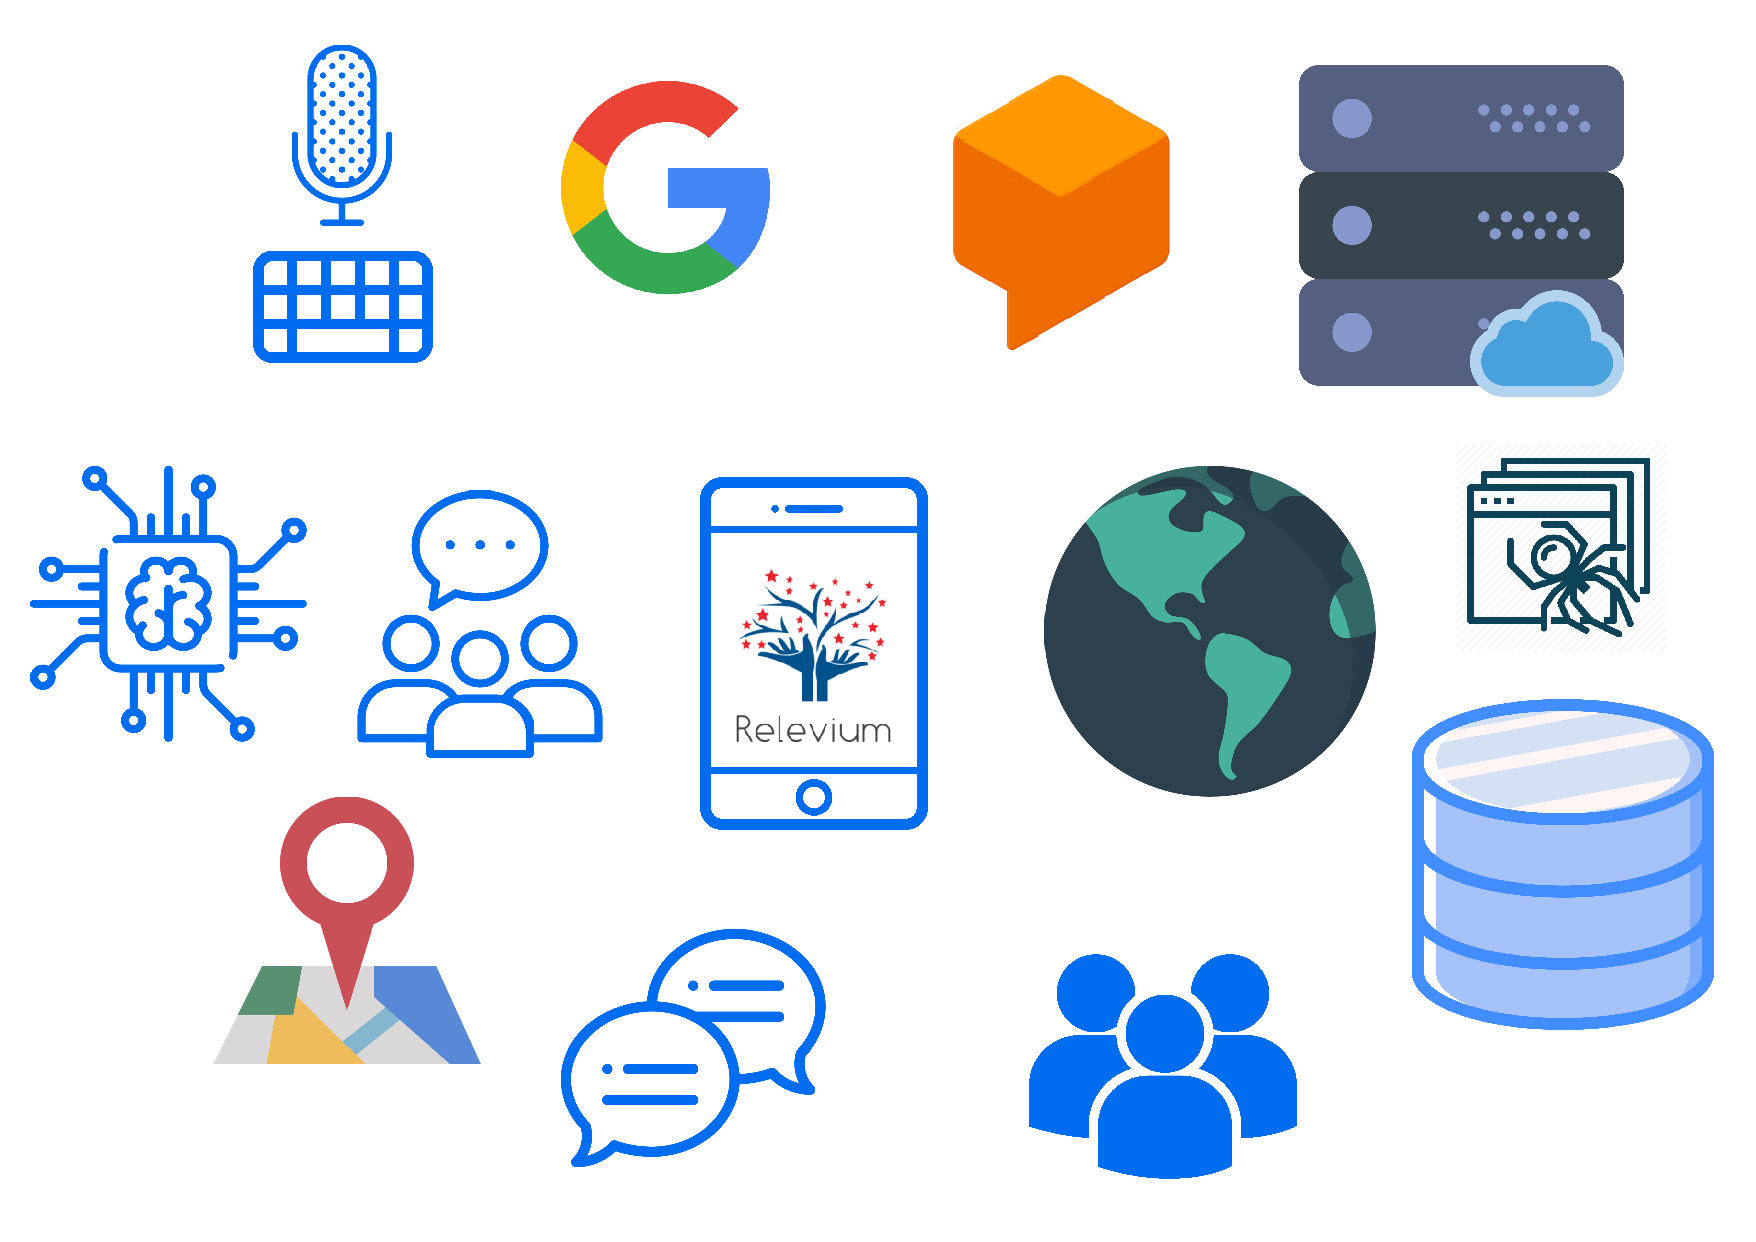
\includegraphics[width=\textwidth]{img3/overview_art.pdf}
    
\end{frame}

% \subsection{Objective}

\begin{frame}{Project Objective}

\begin{itemize}[<+->]
    \item Our main objective is to reduce the number of deaths, injuries and impact from disasters and increase local community and civil society capacity to address the most urgent situations of vulnerability.
    
    \item We also provide individuals, families, and their neighbors with the information they need to stay safe anywhere, anytime.
    \end{itemize}    
\end{frame}


% \subsection{Related work}


\begin{frame}{Related Work}{Emergency \& Disaster Survival Guide}

\begin{columns}

\begin{column}{0.4\linewidth}

Emergency preparedness \& Disaster Survival Guide is paid mobile application that cover almost all the how to survive a disastrous situation with simple  illustrations and written guides.


\end{column}

\begin{column}{0.4\linewidth}

\includegraphics<1>[width=\textwidth]{appImages/EPD1.jpg}
\includegraphics<2>[width=\textwidth]{appImages/EPD2.jpg}

\end{column}

\end{columns}

    
\end{frame}
   
\begin{frame}{Related Work}{Disaster Alert\textsuperscript{\texttrademark}}

\begin{columns}


\begin{column}{0.4\linewidth}
Disaster Alert is a free, mobile app that provides individuals, families, and their loved ones with the information they need to stay safe anywhere in the world. Disaster Alert offers near real-time updates about 18 different types of active hazards as they are unfolding around the globe.
\end{column}

\begin{column}{0.4\linewidth}
    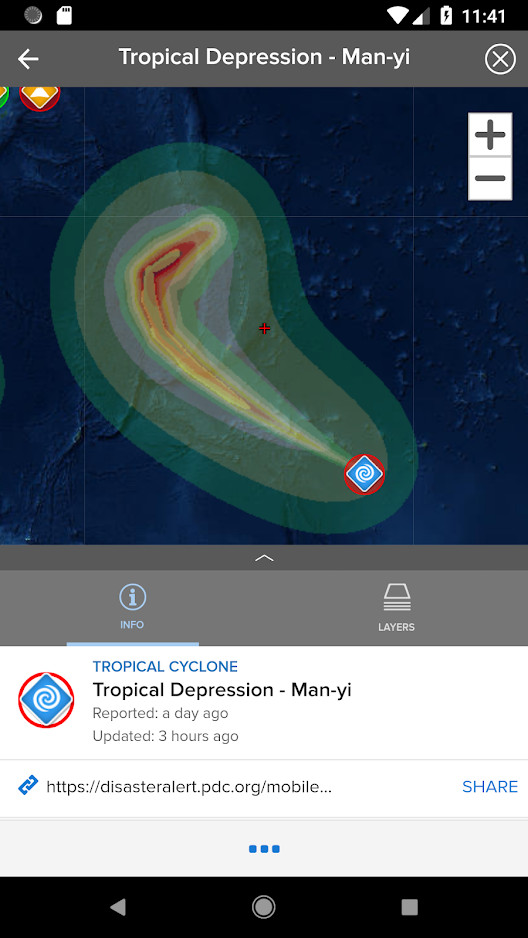
\includegraphics[width=\textwidth]{appImages/DA1.jpg}
\end{column}
\end{columns}

\end{frame}


\section{Requirements}

\subsection{Functional}

\begin{frame}{Relevium Watchful Smart Helper}

\begin{itemize}
    \only<1-2>{
    \item<1-> Communicate with the application through phone's built-in assistant.
    We create intents in the agent that map user input to responses. In each intent, we define examples of user requests that can trigger the intent, what to extract from the request, and how to respond.

    \item<2-> Generally, an intent represents one dialog turn within the conversation. The agent would match that input to its corresponding intent and return the response defined within that intent. The agent’s response usually prompts users for another utterance, which the agent will attempt to match another intent, and the conversation continues.}
    
    \only<3>{\item Relevium project uses Watchful Smart Helper as a advanced way to communicate with user. When the user log-in user will receive a welcome intent from pre-populated text responses.}
\end{itemize} 

\end{frame}

\begin{frame}{Voice Recognition}

Relevium project uses voice recognition as an alternative way to carry out the communication  with  the  user,  we  use  it  because  of  sometimes  the  user  in  critical  situations won’t be able to use the typing method to use the Relevium mobile app, it also enhance the communication and offer the user a variety of different possible ways to use them as input method or interaction ways with our application.

\end{frame}

\begin{frame}{Network of mobiles during the disaster (MANET)}{Stands for ``Mobile Ad-hoc Network"}
\only<1>{
\textit{Connect users in the same geographical area using a wireless mesh network (WMN).}


A MANET is a type of ad-hoc network that can change locations and configure itself on the fly. Because MANETS are mobile, they use wireless connections to connect to various networks. This can be a standard Wi-Fi connection, or another medium, such as a cellular or satellite transmission.}
\only<2>{

\begin{itemize}
    \item The usability of this feature in Relevium project will occur when the infrastructure of the cellular network or WLAN isn’t available or accessible,  so we can make the users who  have  Relevium  mobile  app  communicate  with  their  mobiles  using  Mobile  ad-hoc network (MANET) to share knowledge and current situation that’s happening at each person side, and to help society collaborate and quick help each other during disasters.
\end{itemize}
}
\end{frame}

\begin{frame}{Paramedic User}

\begin{itemize}
    \only<1>{\item 
    One of the most important features During the disaster. When the user register to our application user will be asked to fill a form to prove that the user a paramedic or not (optional), and if user fill this field, then user required to prove that by a picture for work identity or any document prove that user have the right to work with a paramedic degree.}

    \only<2>{\item 
    There may be conditions under which the paramedic user will decide to get away or to be there to help others, there are no conditions for user to follow, he has full freedom to choose what he wants to do by helping others or escape in case of danger.}
    

\end{itemize} 

\end{frame}

\begin{frame}{Shelter users \& Highlight danger zones}


When our application recognizes the user in probable disaster zone then application will disseminate visual and audio disaster warning and evacuation guideline including shortest path of shelter on the map of the application.
    
\end{frame}

\begin{frame}{Share user's location \& information}

\only<1-4>{
Relevium can tell user when a friend is nearby.
\begin{itemize}
    \item<2-> it lets you ``wave" at them and gives you the option to send a message if they wave back.
    \item<3-> it even let you tell your friends where you are and give them directions to your location.
    \item<4-> It will also let you pick a special friend (like a family member, spouse or love interest, for example) to share your location with long-term.
    \end{itemize}
    }
\end{frame}


\begin{frame}{Evacuation Plan}
\begin{itemize}[<+->]

    \item Find shortest safe path to evacuate and override traffic rules if necessary.

    \item The country may lack effective disaster preparedness system to confront natural disasters. Timely disaster warning and evacuation guideline can save lives. In addition, a tourists may face difficulties in finding safe area or shelter prior to the occurrence of natural disasters.
\end{itemize} 
\end{frame}



\begin{frame}{Early alerting system}

Predict hazardous environments and alert users.

The system leverage a third-party Disaster Management Server (DMS), mobile device with our application installed on it and Connect DMS to get updates about disaster (tsunami, cyclone or flood) to get automatic notification of upcoming disaster.
    
\end{frame}


\begin{frame}{Web crawler to collect data from websites}
\only<1>{
A Web crawler is an Internet bot which helps in Web indexing. They crawl one page at a time through a website until all pages have been indexed. Web crawlers help in collecting information about a website and the links related to them, and also help in validating the HTML code and hyperlinks.

\begin{block}{Also Known As}
A Web crawler is also known as a Web spider, automatic indexer or simply crawler.
\end{block}


}
\only<2-3>{
\begin{itemize}
    \item<2-> Web crawlers collect information such the URL of the website, the meta tag information,the Web page content, the links in the web page and the destinations leading from those links, the web page title and any other  relevant information.
    
    \item<3->They  keep  track  of  the URLs which have already been downloaded to avoid downloading the same page again. A combination of policies such as re-visit policy, selection policy, parallelization policy and  politeness  policy  determine  the  behavior  of  the  Web  crawler.
    

\end{itemize}
}

    % \only<4>{ There  are  many challenges  for  web  crawlers,  namely  the  large  and  continuously  evolving  World  Wide Web, content selection trade-offs, social obligations and dealing with adversaries. Web crawlers are the key components of Web search engines and systems that look into web pages.  Web crawlers are also used in data mining, wherein pages are analyzed for different properties like statistics, and data analytic are then performed on them.
    % }

\end{frame}

\subsection{Non-Functional}

\begin{frame}{Safety Requirements}

User agrees by using this system that under no circumstances or any theories of liability under international or civil, common or statutory law including but not limited to strict liability, negligence or other tort theories or contract, patent or copyright laws, will the system be liable for damages of any kind occurring from the use of this system or any information, goods or services obtained on this website including direct, indirect, consequential, incidental, or punitive damages (even if the system has been advised of the possibility of such damages), to the fullest extent permitted by law.
    
\end{frame}

\begin{frame}{Security Requirements}
    
\begin{itemize}
    \item<1-> This application will have users credentials like (mobile numbers, addresses ..etc)
So it must have encrypted personal data and the chat between users should be encrypted too.

    \item<2-> Some of the supposed algorithms to be used are: \textbf{AES-256, ARC4, RSA-2048}.
% \hrulefill


    \item<3-> Other ``external" factors which can be used alongside the user’s identification to securely reset a password may be SMS or physical keys (YubiKey).
    \end{itemize}
\end{frame}


\begin{frame}{Software Quality Attributes}
    \begin{itemize}
    \item<1-> The application should guarantee availability as it will be available every time and it must maintain lowest MTBF (mean time between failure).
    
    \item<2-> It must meet correctness because any misinformation could lead to dangerous situation for the user. 
    \item<3-> It should be flexible to be used easily in hard times, also it should offer the testers an instructions about how the application should be tested and what is the correct input and output.
    
    \item<4-> It also should be adaptable to any environment changes, app must meet portability condition as it used in a critical situations, the last but not least is the maintainability concern and it should be maintained at least one time per week.
    \end{itemize}
\end{frame}


\section{Constraints}

% \subsection{Solution}

\begin{frame}{Solution Constrains}

\begin{itemize}
    \item<1-> Due to the choice of technology, some constraints have arisen mainly in the web crawling section.  To start, a crawler must wait between repeated accesses to the same website. 

    \item<2-> Otherwise,  the crawler can be blocked.  In addition,  duplicate content can generate a waste of valuable resources.
\end{itemize}
\end{frame}


% \subsection{Memory \& Space}

\begin{frame}{Memory \& Space Constrains}
Our application run on mobile devices with very limited hardware specs which may lead to overheating or battery drain, above all that it will be limited to small amount of ram and storage space on some devices. 

\end{frame}

% \subsection{Policy \& Privacy}
\begin{frame}{Policy \& Privacy}

\begin{itemize}
    \item<1-> The application tries to use all the available mobile resource in disastrous times to save all the user in potential danger eg: using the phone while it's on standby mode to alert the user or use mobile flash to help users who are stuck under derbies.
    
    \item<2-> Although we do our best to save the user life, this does not mean we will prevent their death 100\%, which is must be stated to clear us from any charges.
\end{itemize}    
\end{frame}

% \subsection{Schedule}
\begin{frame}{Schedule Constrains}
\begin{exampleblock}{Release}
    The project has a relatively small time-frame. Therefore, the time is a major concern. \linebreak The project should be functioning and completed by the mid of 2019.
    \end{exampleblock}
\end{frame}


\begin{frame}{Assumption}

Main assumption about the product is that it will always be used on mobile phones that have enough performance. If the phone does not have enough hardware resources available for the application.

For example the users might have allocated them with other applications, there may be scenarios where the application does not work as intended or even at all.
    
\end{frame}



% \begin{frame}{Performance Requirements}
    
% \end{frame}


\section{Analysis Models}

\subsection{Project Schedule}

\begin{frame}{Gantt chart}{Detailed View}
    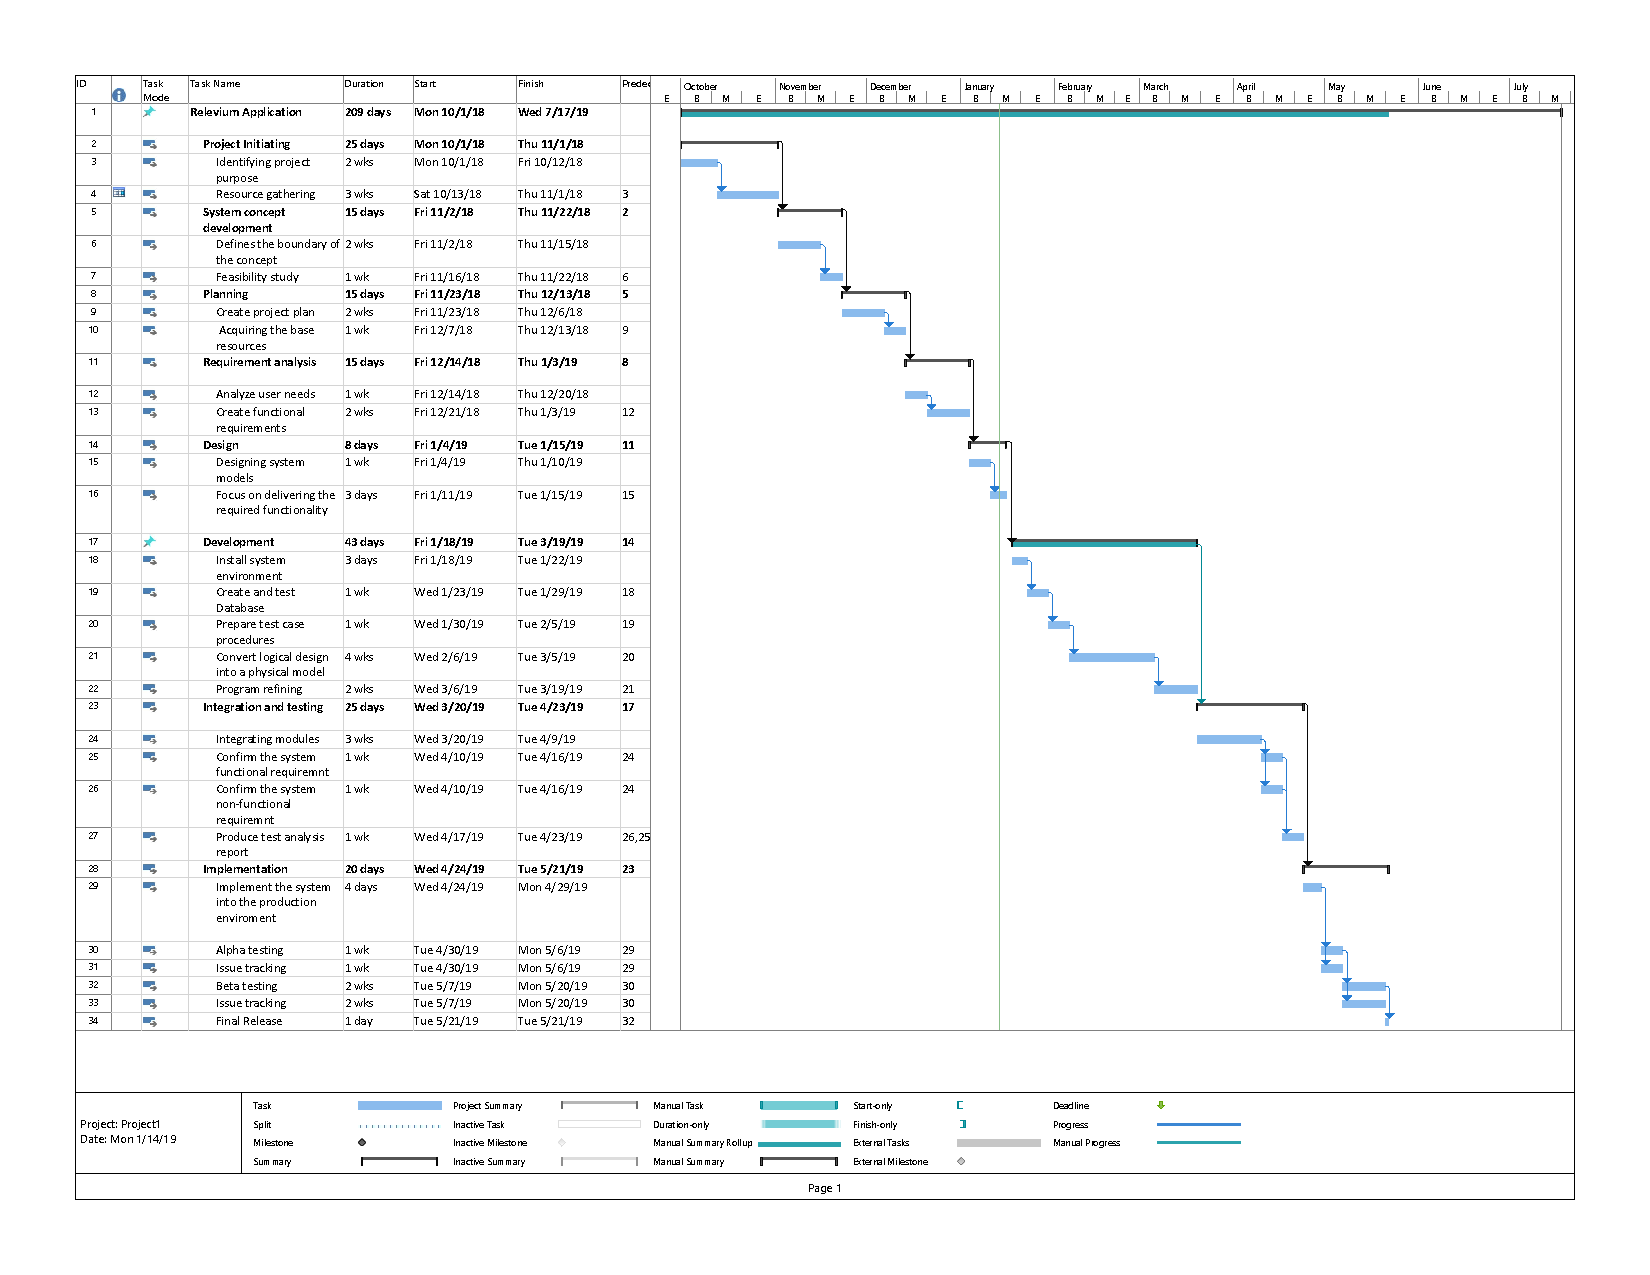
\includegraphics[width=\linewidth]{gantt/gantt_scale.pdf}
\end{frame}


\subsection{Structural}



\begin{frame}{Class Diagram}{Client Domain Logic}
    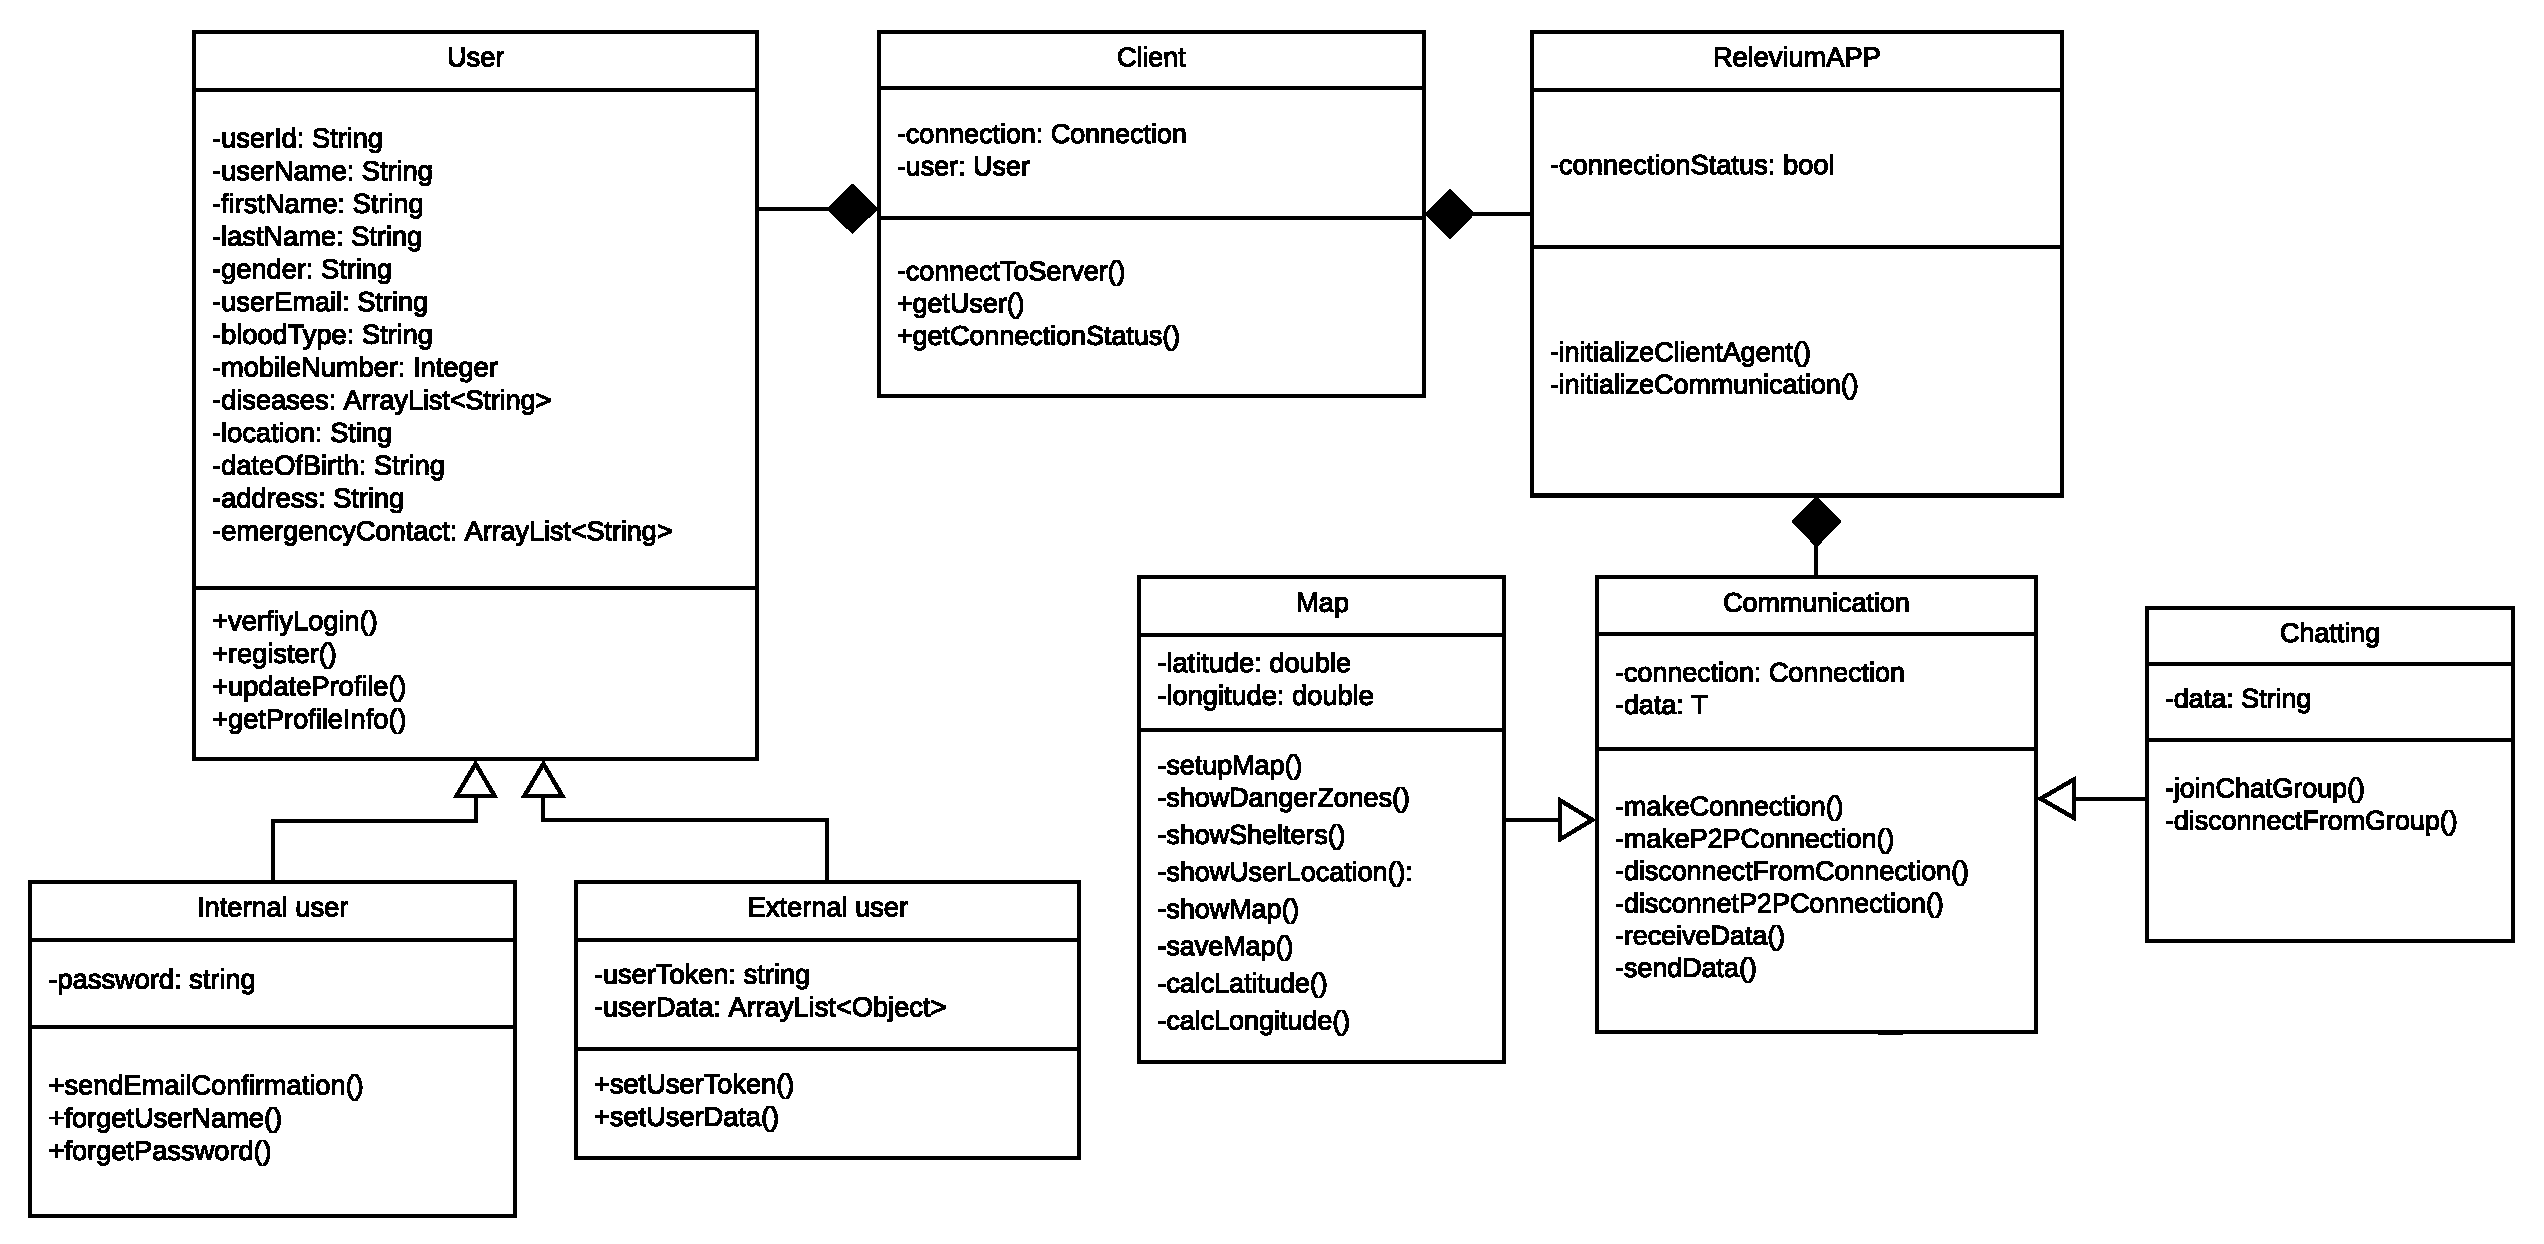
\includegraphics[width=.9\linewidth]{img3/ClassDiagram1.pdf}
\end{frame}

\begin{frame}{Class Diagram}{Client Domain Logic (Cont.)}
    \centering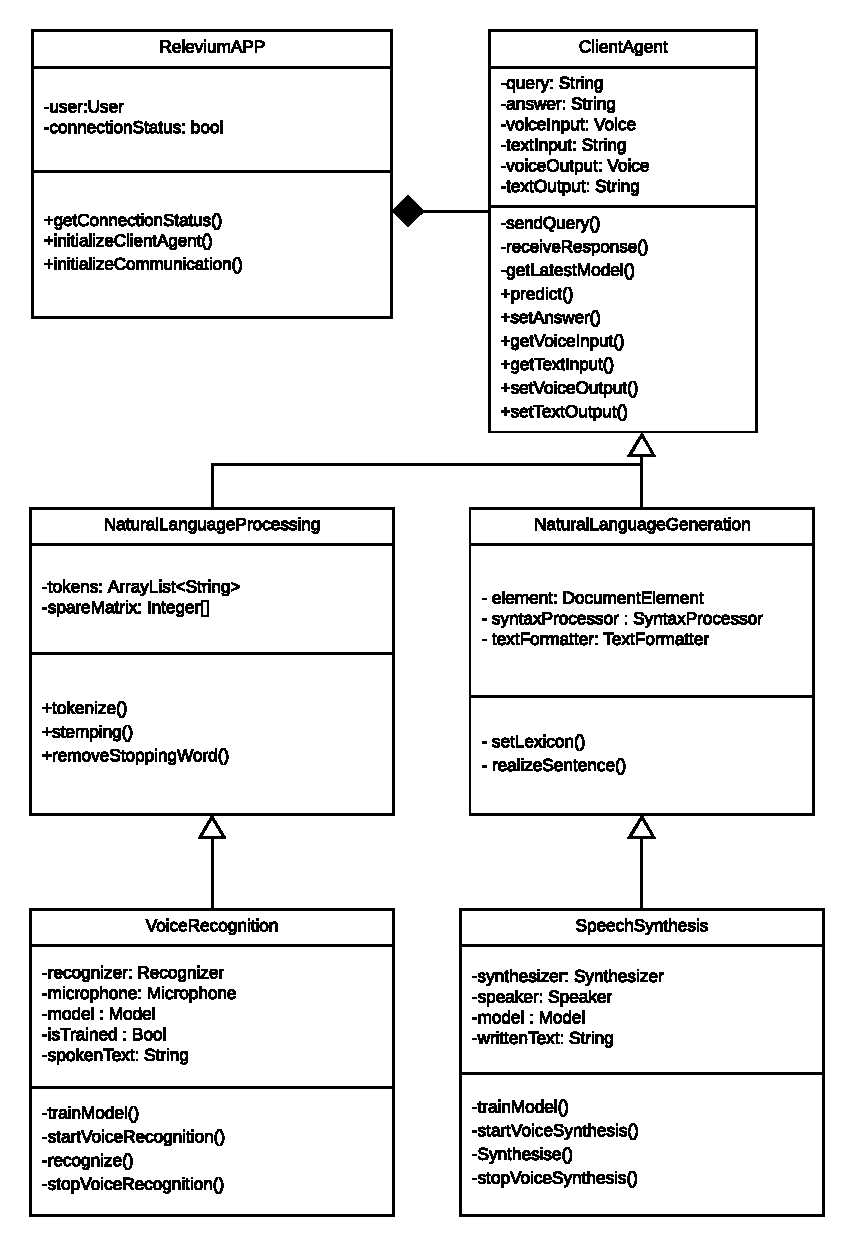
\includegraphics[height=.7\textheight]{img3/ClassDClass1DIV.pdf}
\end{frame}

\begin{frame}{Class Diagram}{Server Domain Logic}
    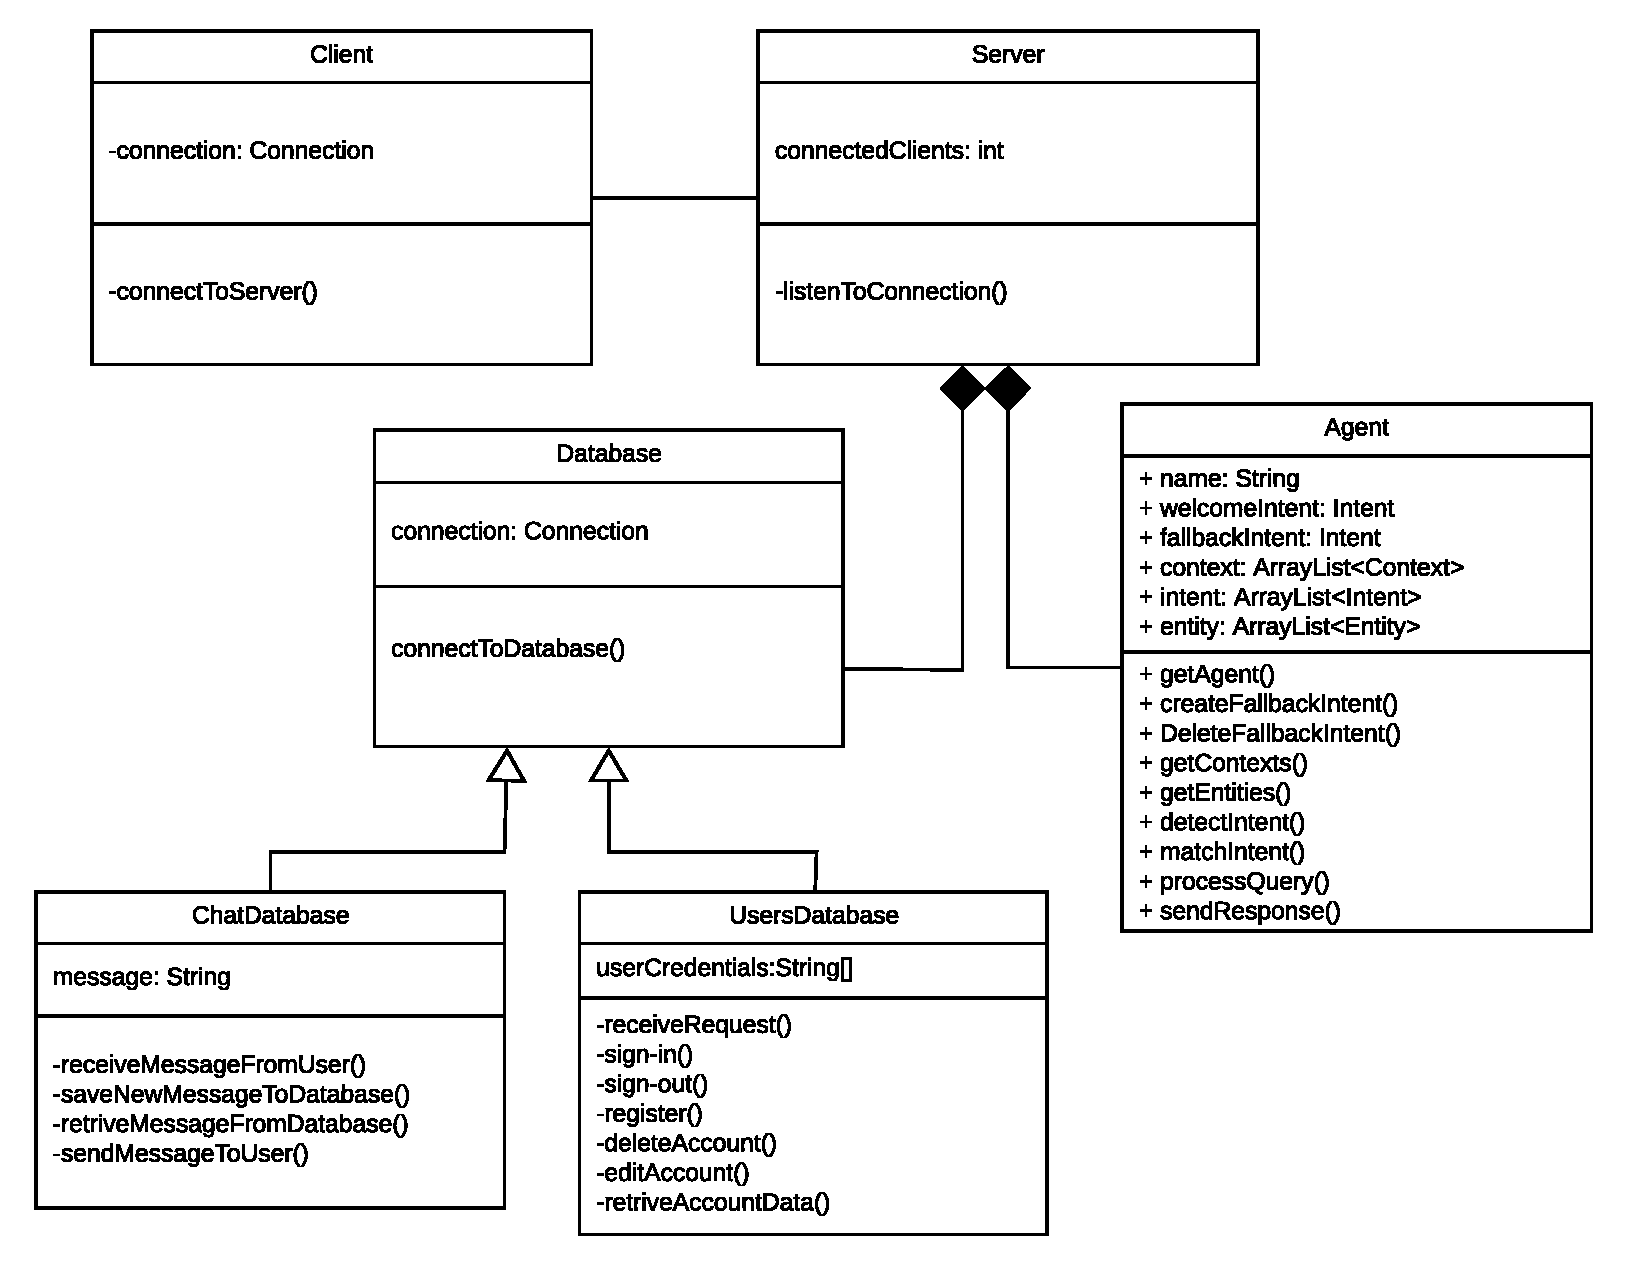
\includegraphics[width=.92\linewidth]{img3/ClassDiagramServerLogic.pdf}
\end{frame}

\begin{frame}{Class Diagram}{Agent Implementation}
    \centering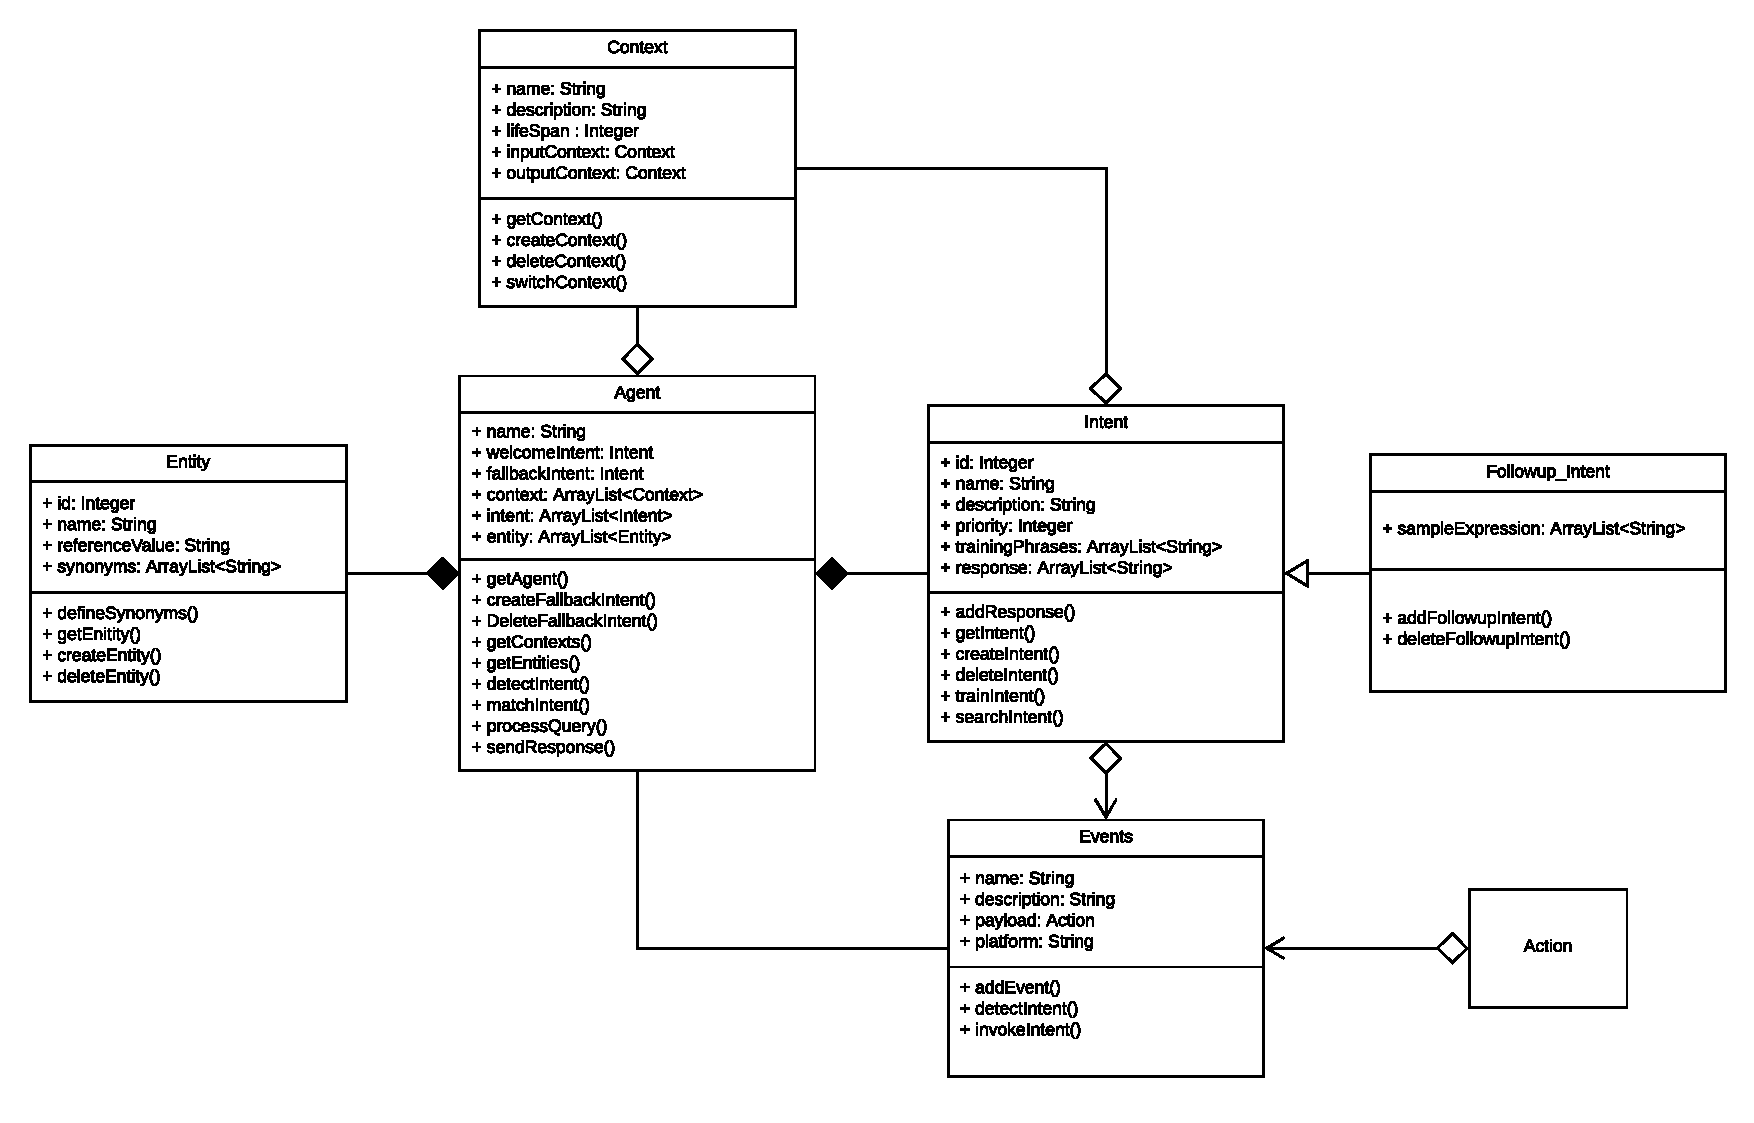
\includegraphics[width=.96\linewidth]{img2/ClassDiagramAgent.pdf}
\end{frame}



\subsection{Behavioural}

\begin{frame}{Sequence Diagram}{Utterance Route}
    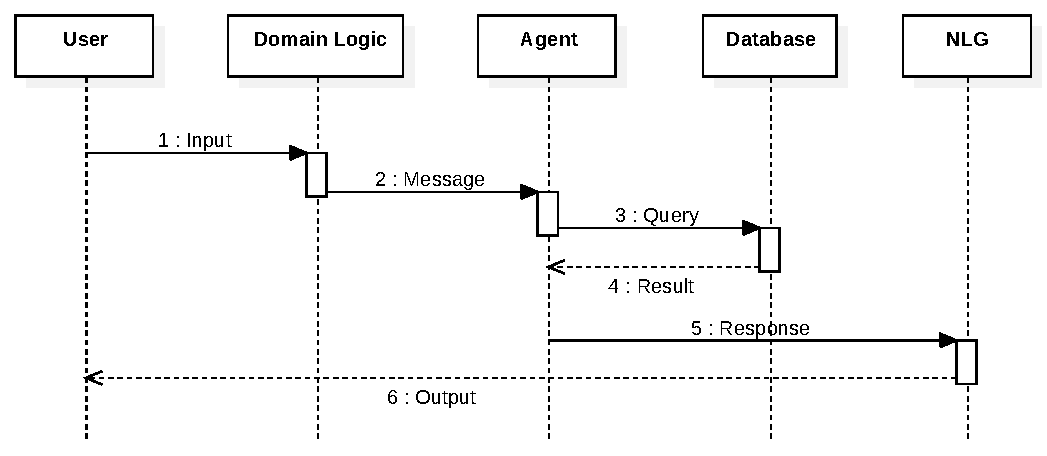
\includegraphics[width=\linewidth]{img3/SequenceDiagram2.pdf}
\end{frame}

\begin{frame}{Sequence Diagram}{Communication Process}
    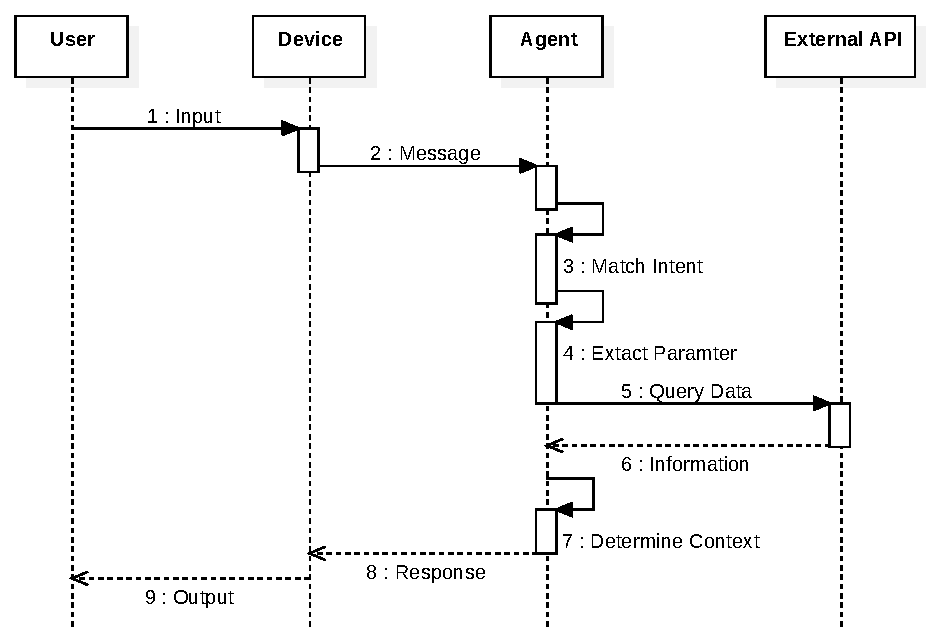
\includegraphics[width=\linewidth]{imgs/SequenceDiagram1.pdf}
\end{frame}

\begin{frame}{State Chart Diagram}{Context Matching}
    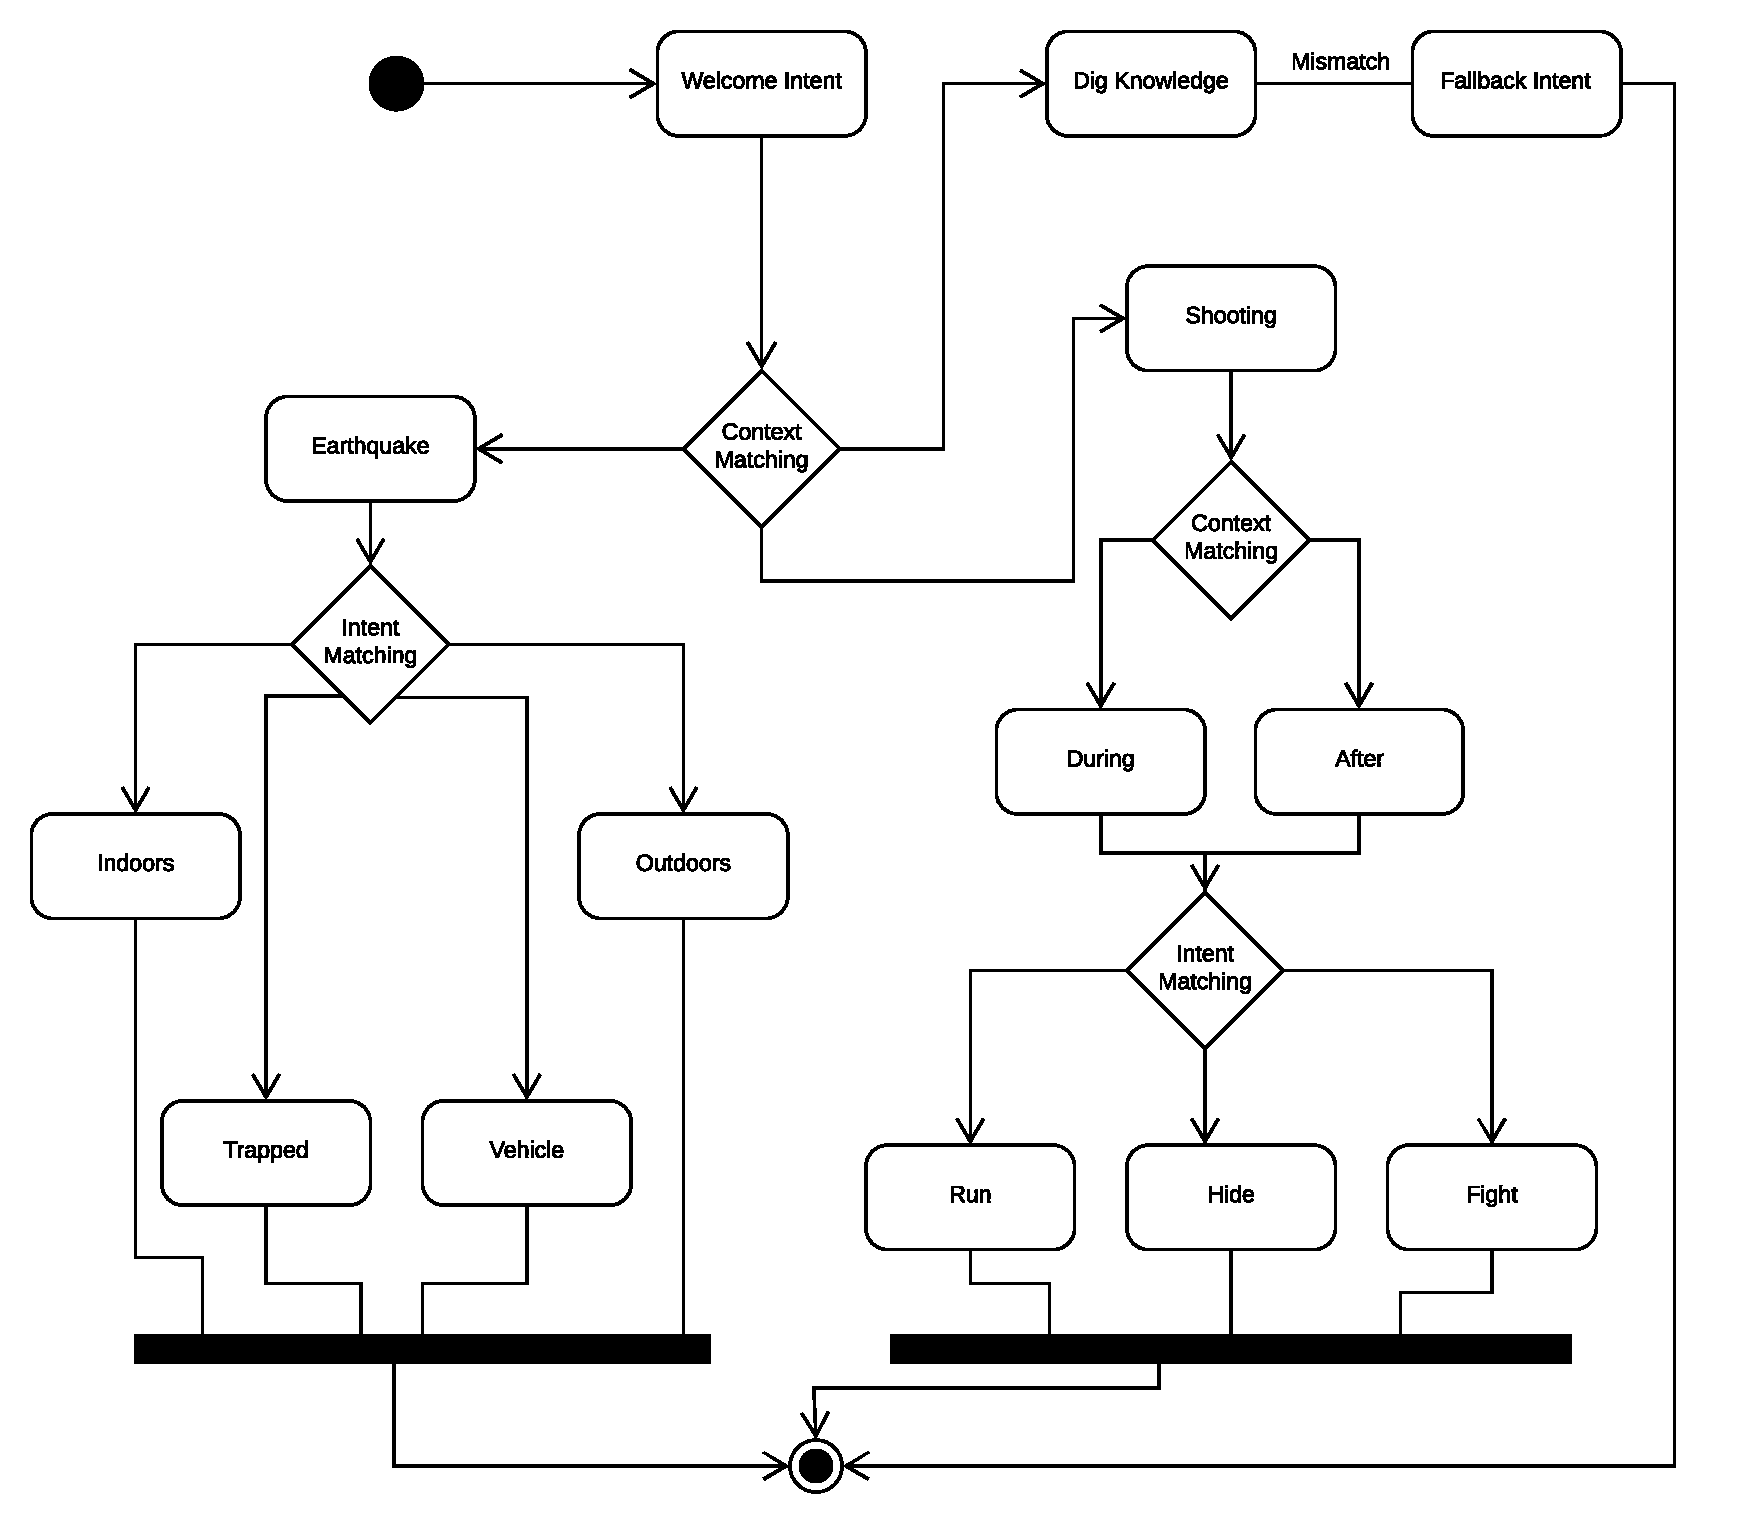
\includegraphics[width=.92\linewidth]{img3/state1.pdf}
\end{frame}

\begin{frame}{State Chart Diagram}{Context Matching (cont.)}
    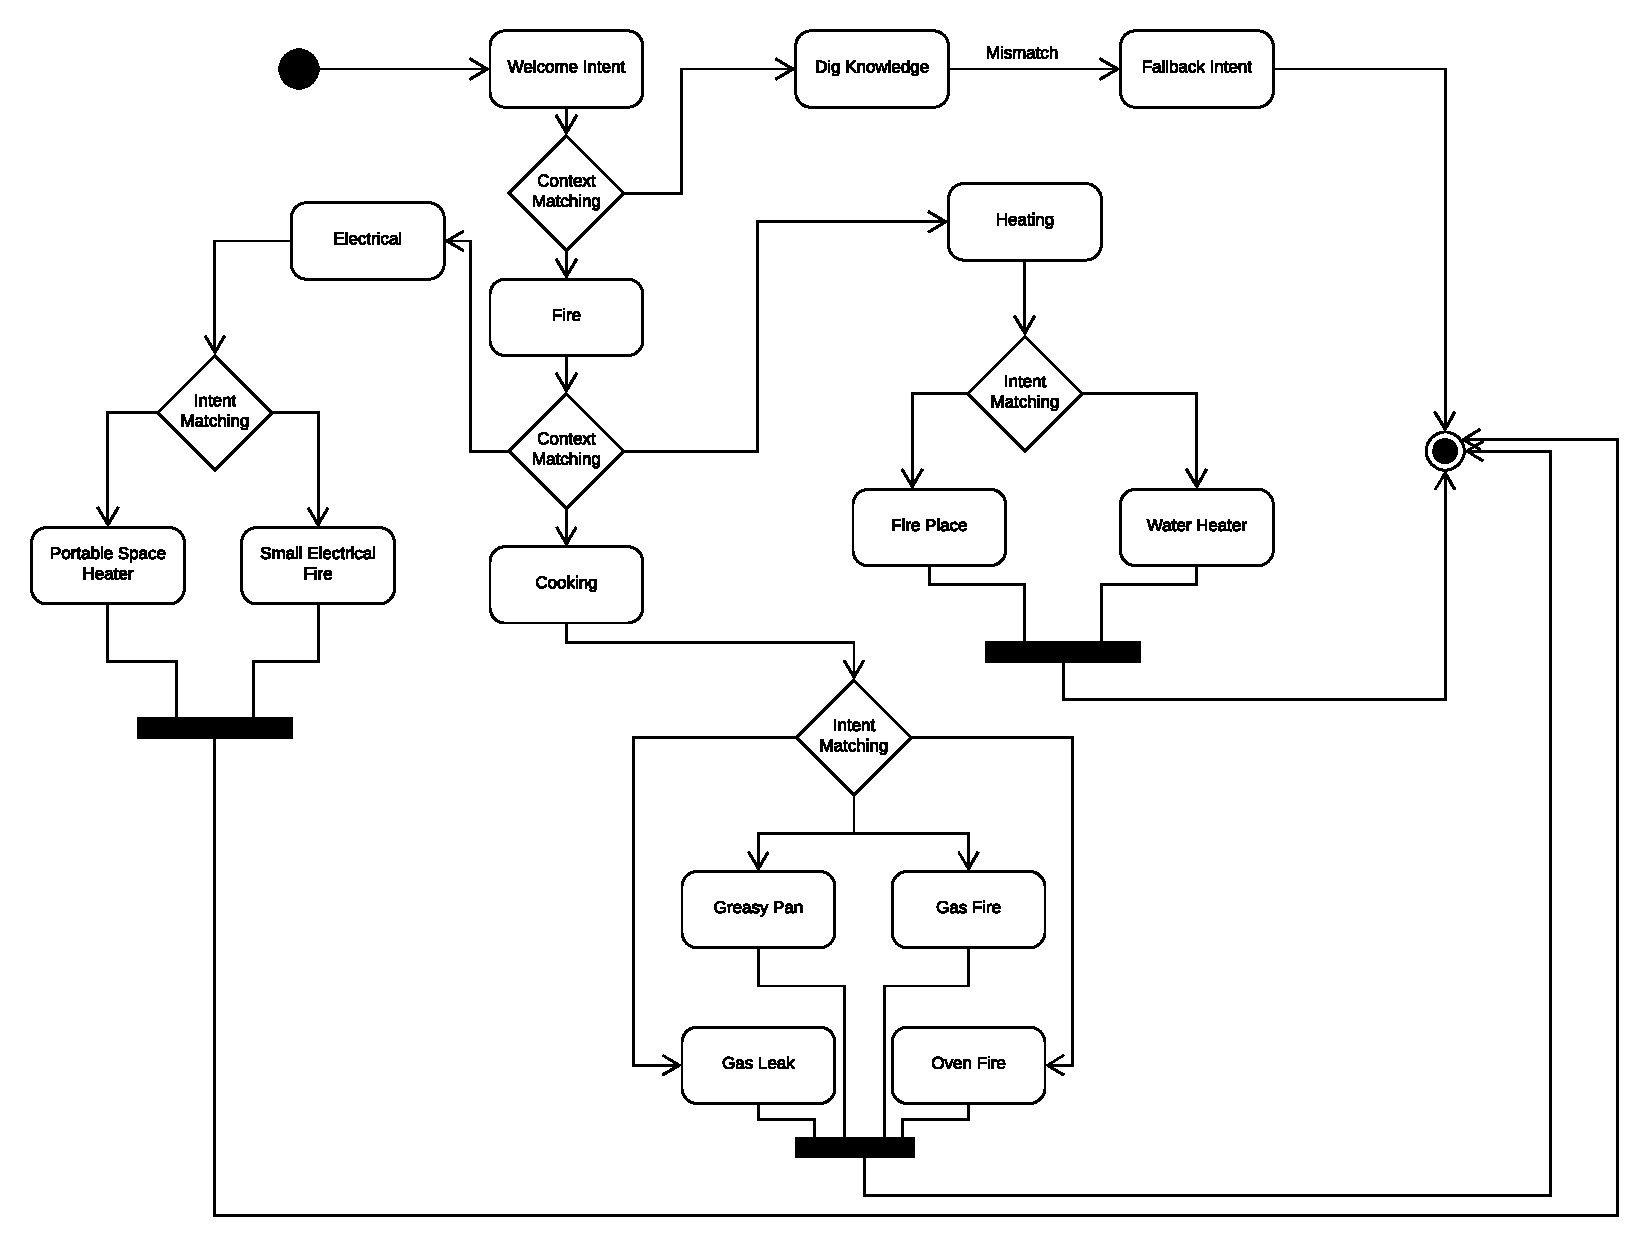
\includegraphics[width=\linewidth]{img3/state2.pdf}
\end{frame}

\begin{frame}{Entity Relationship Diagram}{Crow Notation}
    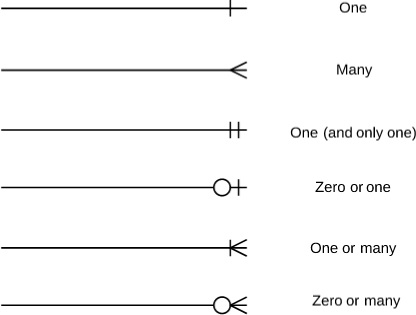
\includegraphics[width=.92\linewidth]{img3/ERD-Notation.jpg}
\end{frame}

\begin{frame}{Entity Relationship Diagram}{User Entity}
    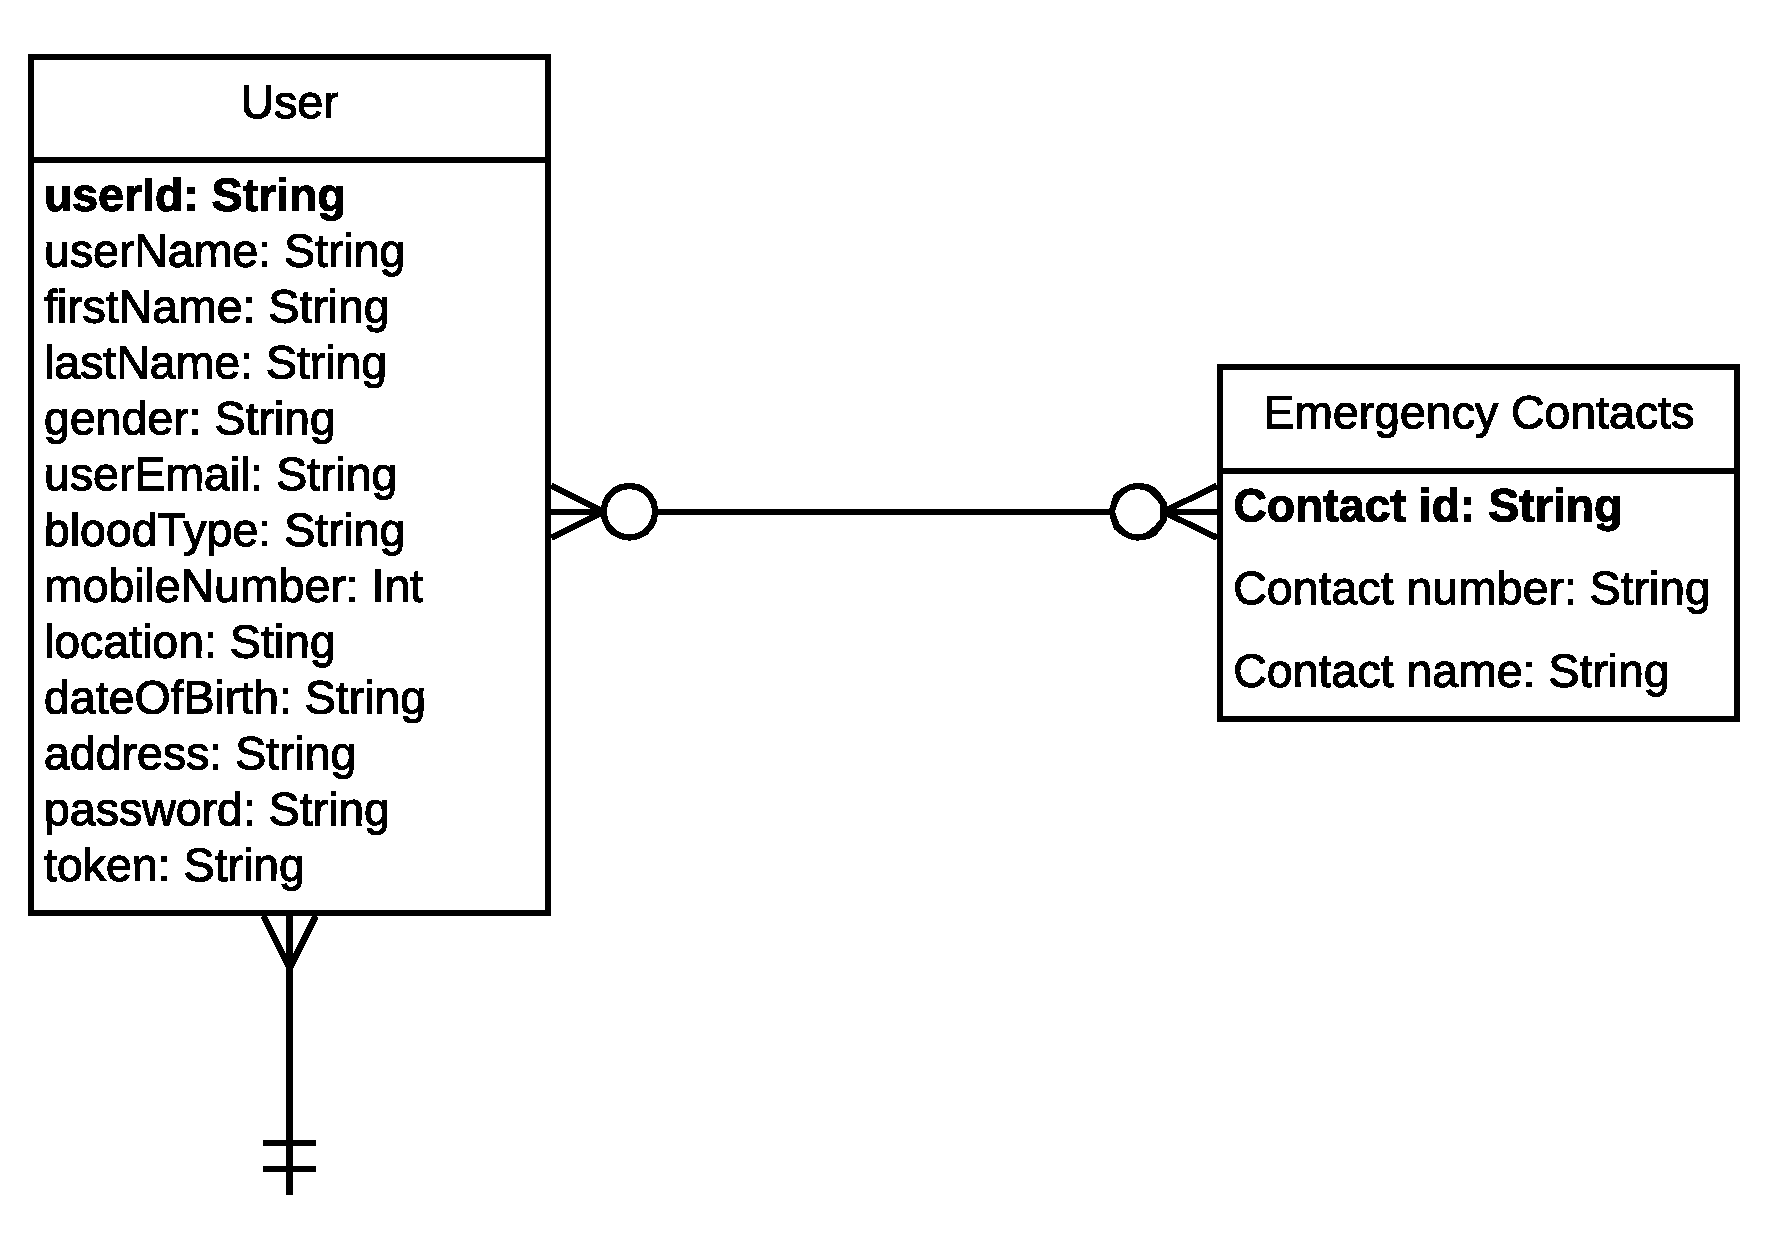
\includegraphics[width=.92\linewidth]{img3/erd1.pdf}
\end{frame}

\begin{frame}{Entity Relationship Diagram}{Agent}
    \centering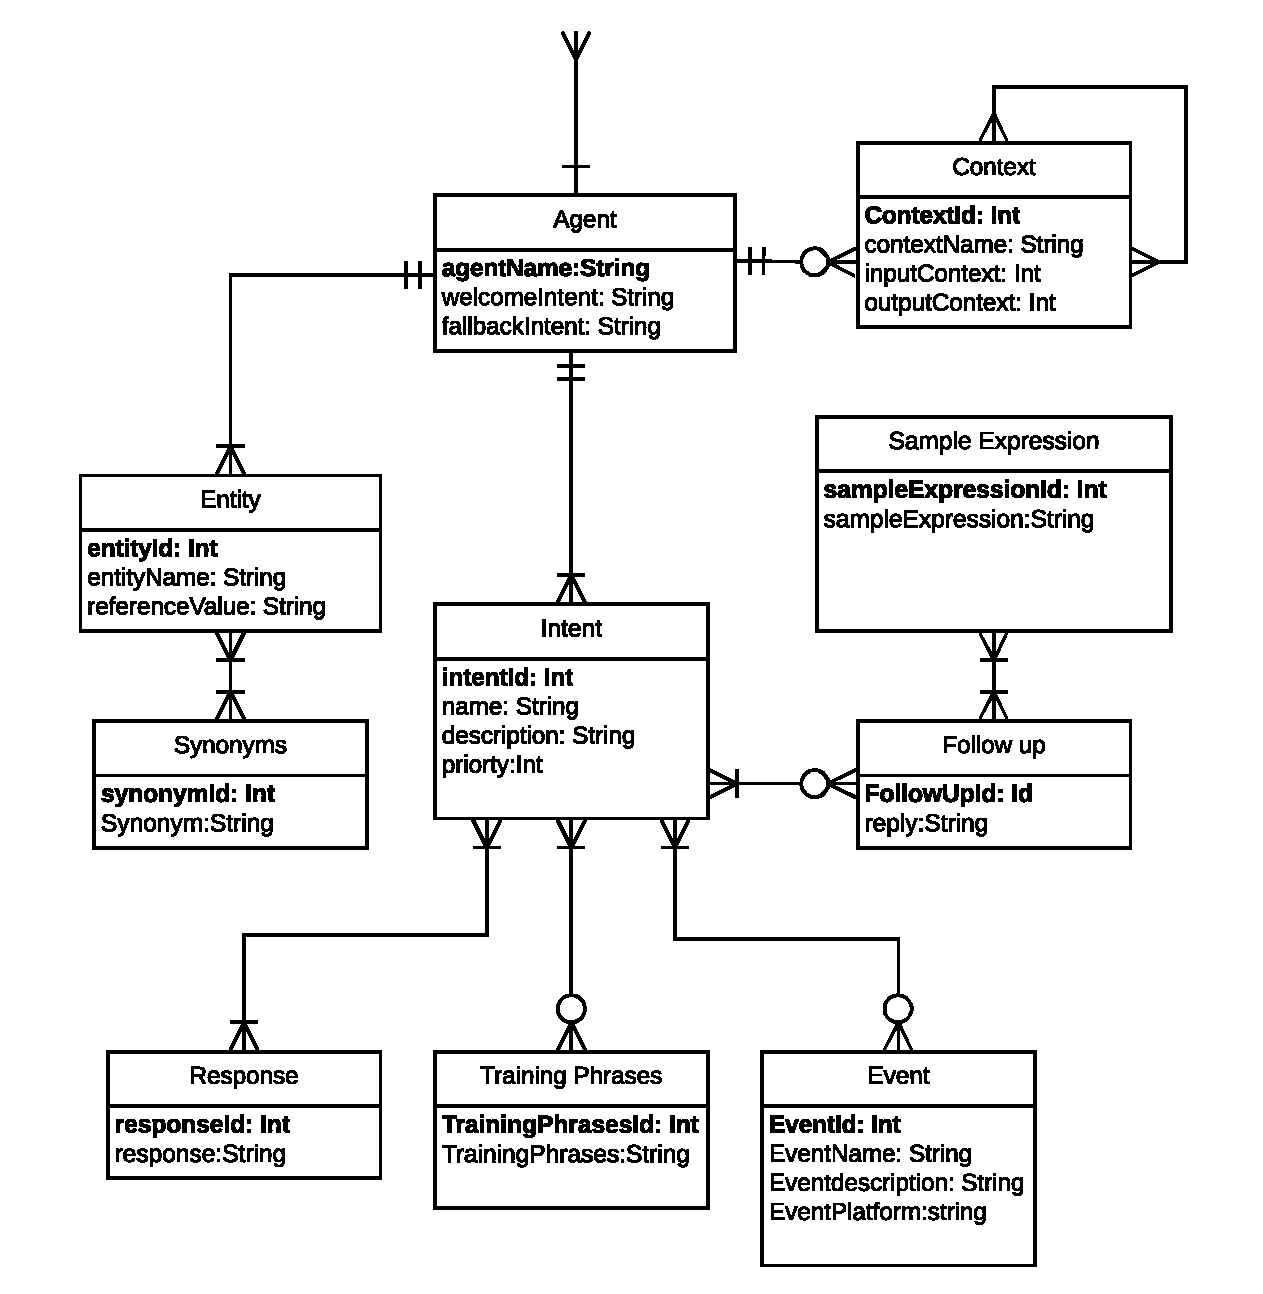
\includegraphics[width=.78\linewidth]{img2/erd2.pdf}
\end{frame}

\begin{frame}{Use Case Diagram}{Application Interaction}
    \centering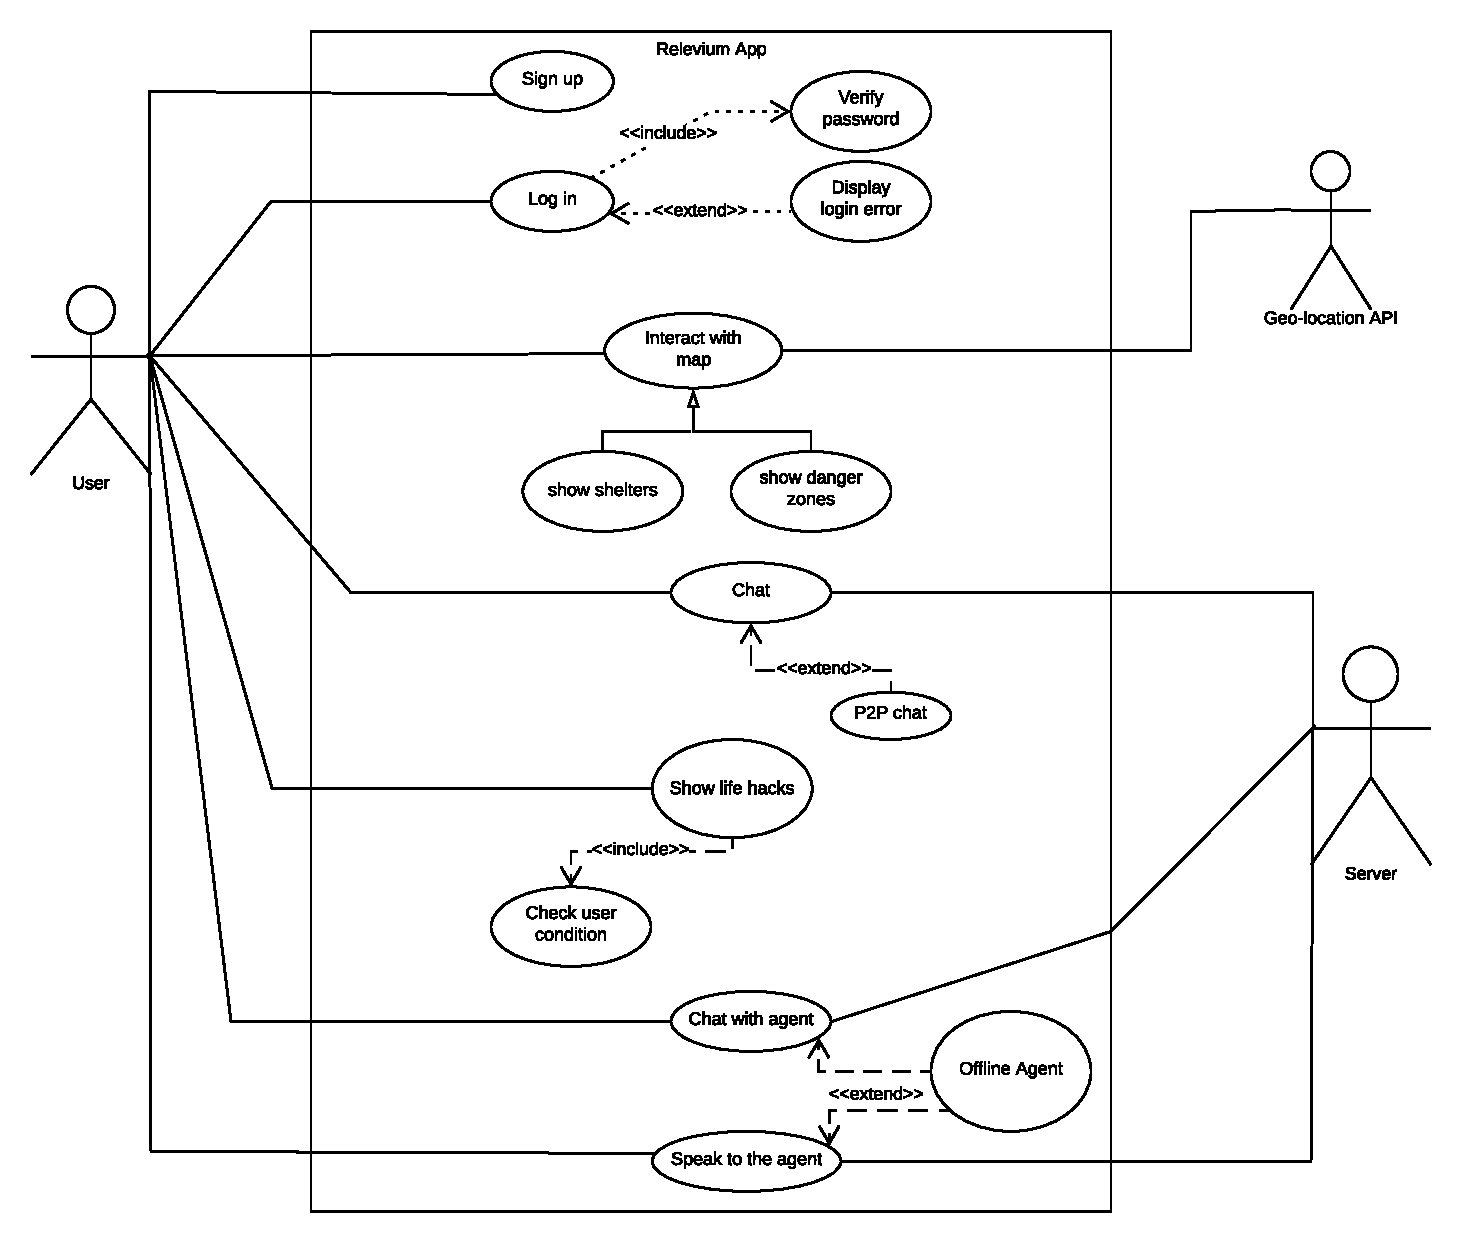
\includegraphics[width=.85\linewidth]{img3/UseCaseDiagram1.pdf}
\end{frame}


\section{AI Approach}
\subsection{DMN}
\begin{frame}{Dynamic Memory Network}

\only<1-3>{
\begin{itemize}[<+->]


\item Most tasks in natural language processing can be cast into question answering (QA) problems over language input.

\item The dynamic memory network (DMN) is a neural network architecture which processes input sequences and questions, forms episodic memories, and generates relevant answers.

\item Questions trigger an iterative attention process which allows the model to condition its attention on the inputs and the result of previous iterations. These results are then reasoned over in a hierarchical recurrent sequence model to generate answers.
\end{itemize}
}

\only<4-8>{
\begin{itemize}
\item The DMN can be trained end-to-end and obtains state-of-the-art results on several types of tasks and datasets:

\begin{enumerate}
    \item<5-> Question answering (Facebook's bAbI dataset). 
    \item<6-> Text classification for sentiment analysis\\(Stanford Sentiment Treebank).
    \item<7-> Sequence modeling for part-of-speech tagging\\ (WSJ-PTB).
\end{enumerate}
\item<8-> The training for these different tasks relies exclusively on trained word vector representations and input-question-answer triplets.
\end{itemize}

}

\only<9>
{
\centering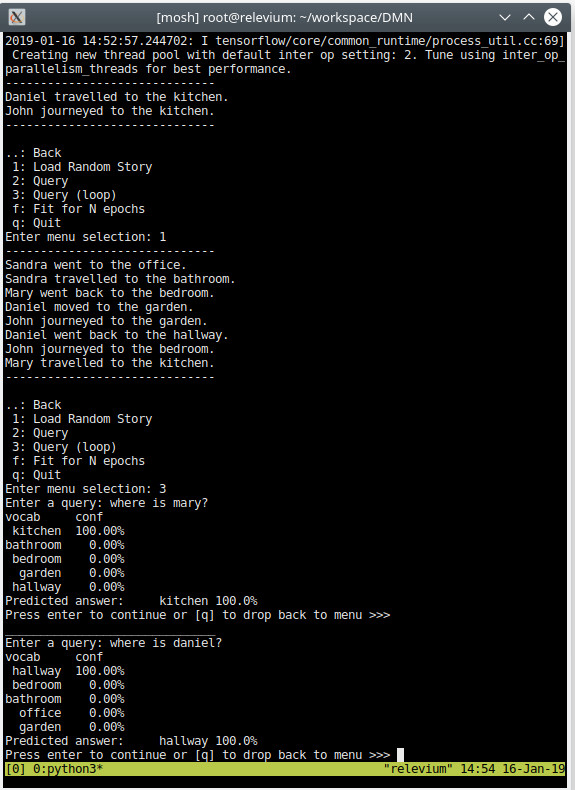
\includegraphics[width=.6\textwidth]{ml_imgs/dmn_crop.jpg}
}
\end{frame}

\subsection{SQuAD}
\begin{frame}{SQuAD}

\only<1>{
\framesubtitle{What is SQuAD?}
\textbf{S}tanford \textbf{Qu}estion \textbf{A}nswering \textbf{D}ataset (SQuAD) is a reading comprehension dataset, consisting of questions posed by crowdworkers on a set of Wikipedia articles, where the answer to every question is a segment of text, or span, from the corresponding reading passage, or the question might be unanswerable.
}

\only<2-3>
{
\framesubtitle{What is SQuAD?}

\begin{itemize}

 \item<2-> SQuAD2.0 combines the 100,000 questions in SQuAD1.1 with over 50,000 new, unanswerable questions written adversarially by crowdworkers to look similar to answerable ones.
 \item<3-> To do well on SQuAD2.0, systems must not only answer questions when possible, but also determine when no answer is supported by the paragraph and abstain from answering. SQuAD2.0 is a challenging natural language understanding task for existing models.
\end{itemize}
}


\only<4>
{
\framesubtitle{Leaderboard - October 2018}
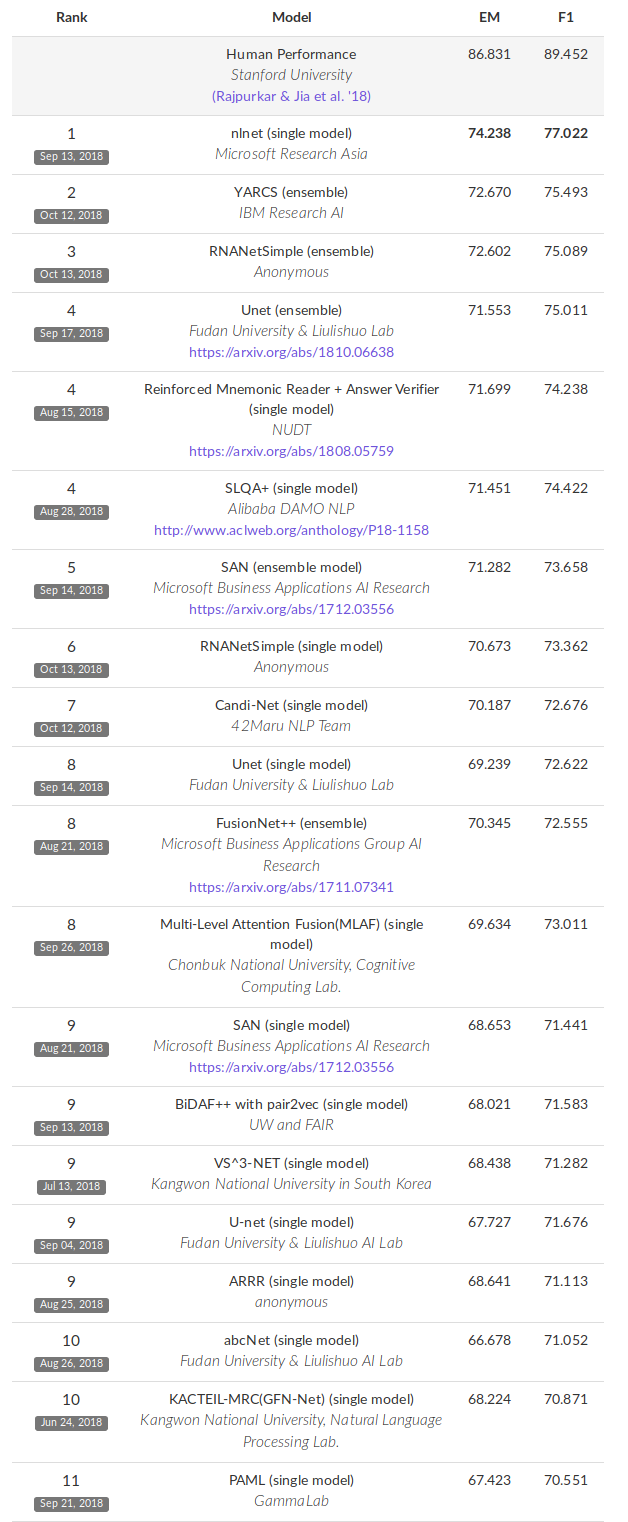
\includegraphics[width=\textwidth]{ml_imgs/squad_oct.png}
}

\only<5>
{
\framesubtitle{Leaderboard - January 2019}
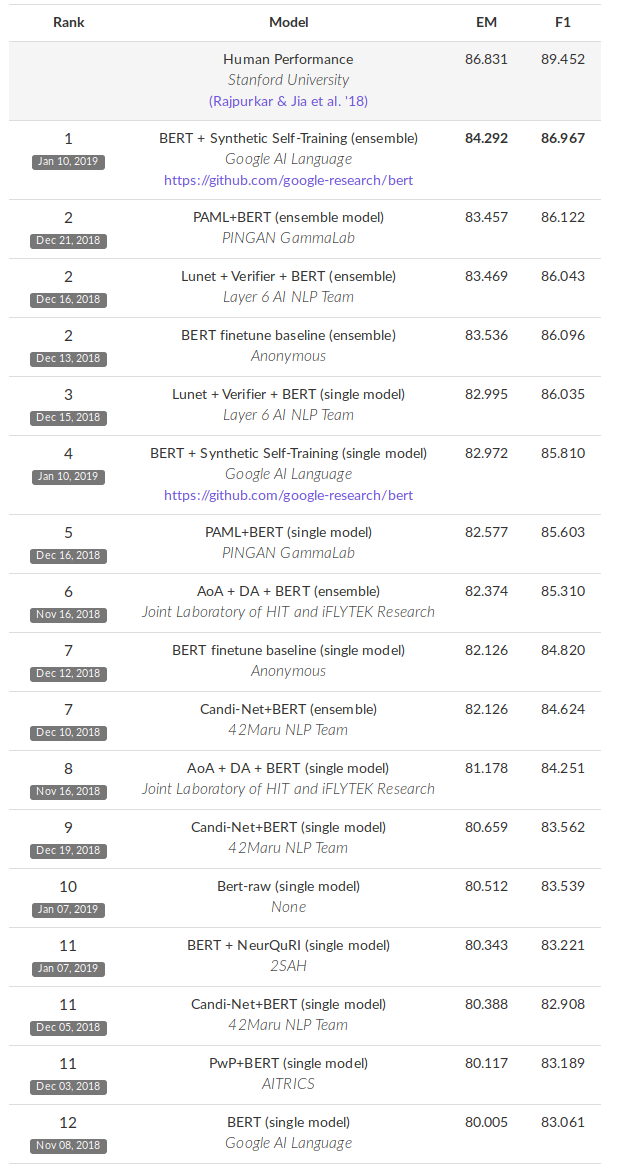
\includegraphics[width=\textwidth]{ml_imgs/squad_jan.png}
}
    
\end{frame}


\subsection{BERT}

\begin{frame}{Deep Bidirectional Transformers for NLP}

\only<1-3>{
\only<1>{
\begin{block}{BERT}
Bidirectional Encoder Representations from Transformers, is a new method of pre-training language representations which obtains state-of-the-art results on a wide array of Natural Language Processing (NLP) tasks.
\end{block}
}
\begin{itemize}
    \item<2-> BERT is a method of pre-training language representations, meaning that we train a general-purpose ``language understanding" model on a large text corpus (like Wikipedia), and then use that model for downstream NLP tasks that we care about (like question answering).

    \item<3-> BERT outperforms previous methods because it is the first unsupervised, deeply bidirectional system for pre-training NLP.
\end{itemize}
}


\only<4-5>{

\only<4>{
\begin{block}{Unsupervised}
Unsupervised means that BERT was trained using only a plain text corpus, which is important because an enormous amount of plain text data is publicly available on the web in many languages.
\end{block}}

\only<5>
{
Pre-trained representations can also either be context-free or contextual, and contextual representations can further be unidirectional or bidirectional. 

Context-free models such as \textbf{word2vec} or \textbf{GloVe} generate a single ``word embedding" representation for each word in the vocabulary, so bank would have the same representation in bank deposit and river bank.

Contextual models instead generate a representation of each word that is based on the other words in the sentence.
}
}


\only<6-7>{
\only<6>{
BERT was built upon recent work in pre-training contextual representations — including Semi-supervised Sequence Learning, Generative Pre-Training, \textbf{ELMo}, and \textbf{ULMFit} — but crucially these models are all unidirectional or shallowly bidirectional. This means that each word is only contextualized using the words to its left (or right).
}

\only<7>{
For example, in the sentence \underline{I made a bank deposit} the unidirectional representation of bank is only based on \underline{I made a} but not \underline{deposit}. Some previous work does combine the representations from separate left-context and right-context models, but only in a ``shallow" manner.


BERT represents ``\underline{bank}" using both its left and right context — \underline{I made a ... deposit} — starting from the very bottom of a deep neural network, so it is deeply bidirectional.}
}

\only<8-10>
{

BERT-Base, Multilingual Cased: 104 languages, 12-layer, 768-hidden, 12-heads, 110M parameters


\only<9>{
\begin{itemize}
\item Pre-training is fairly expensive (four days on 4 to 16 Cloud TPUs), but is a one-time procedure for each language (current models are English-only). They are releasing a number of pre-trained models from the paper which were pre-trained at Google. Most NLP researchers will never need to pre-train their own model from scratch.
\end{itemize}
}

\only<10>{
\begin{itemize}
\item Fine-tuning is inexpensive. All of the results in the paper can be replicated in at most 1 hour on a single Cloud TPU, or a few hours on a GPU, starting from the exact same pre-trained model. SQuAD, for example, can be trained in around 30 minutes on a single Cloud TPU to achieve a Dev F1 score of 91.0\%, which is the single system state-of-the-art.
\end{itemize}
}


}
\end{frame}

\section{Business Model}

\begin{frame}{Business Model}

\only<1>{
\framesubtitle{Definitions}
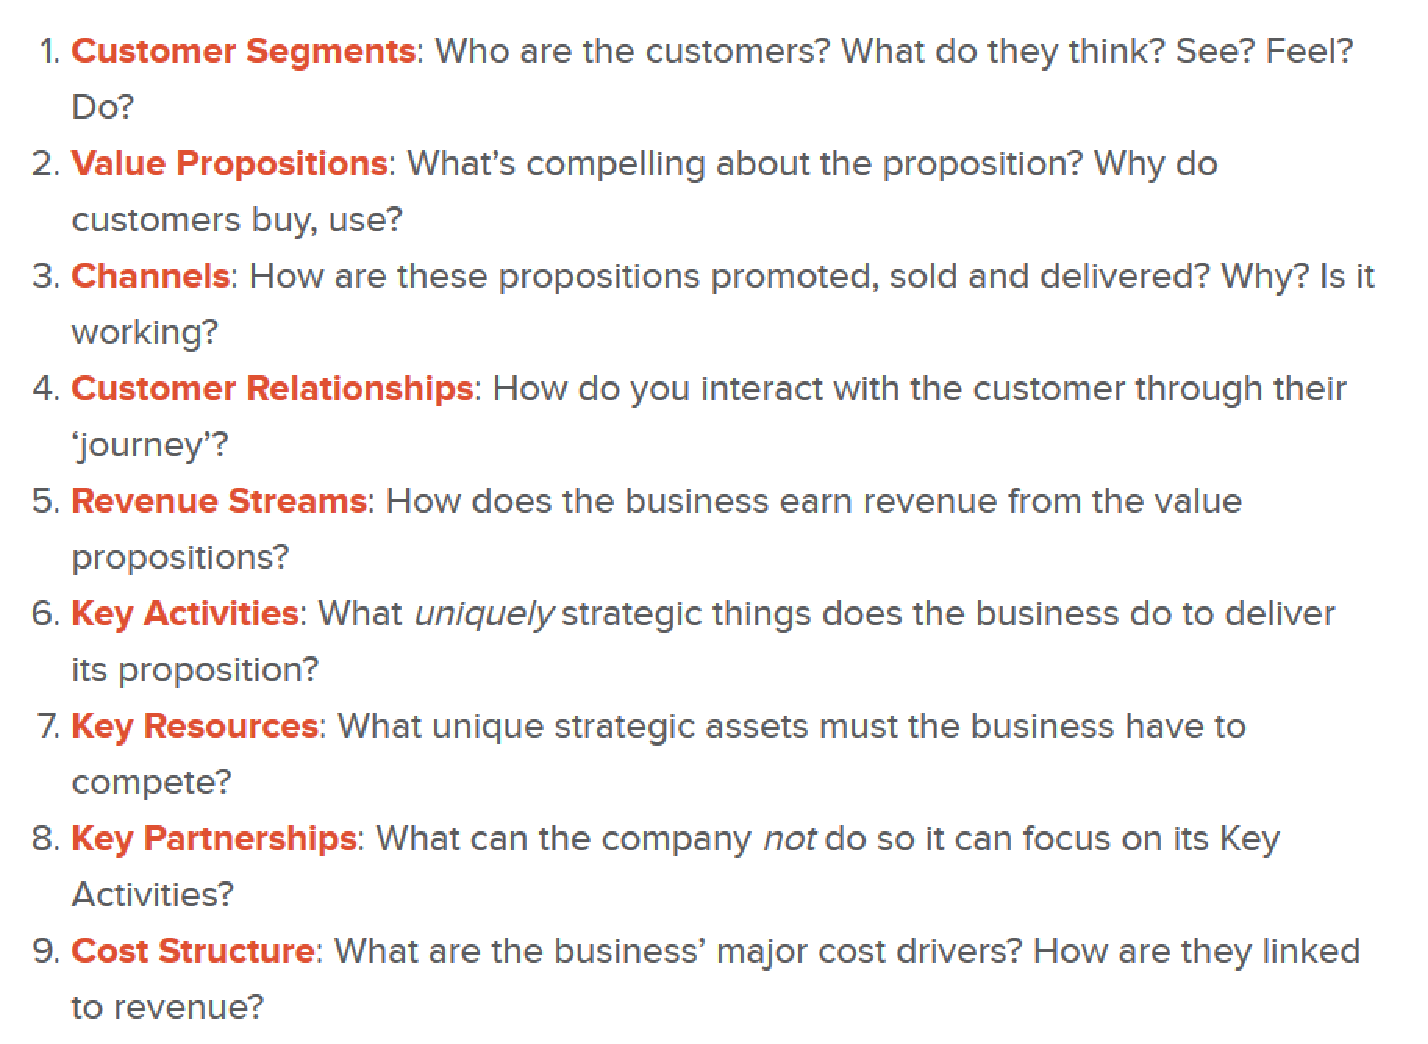
\includegraphics[height=.7\textheight]{img3/Bussiness_model_nine_elements.pdf}
}

\only<2>{
\framesubtitle{Canvas}

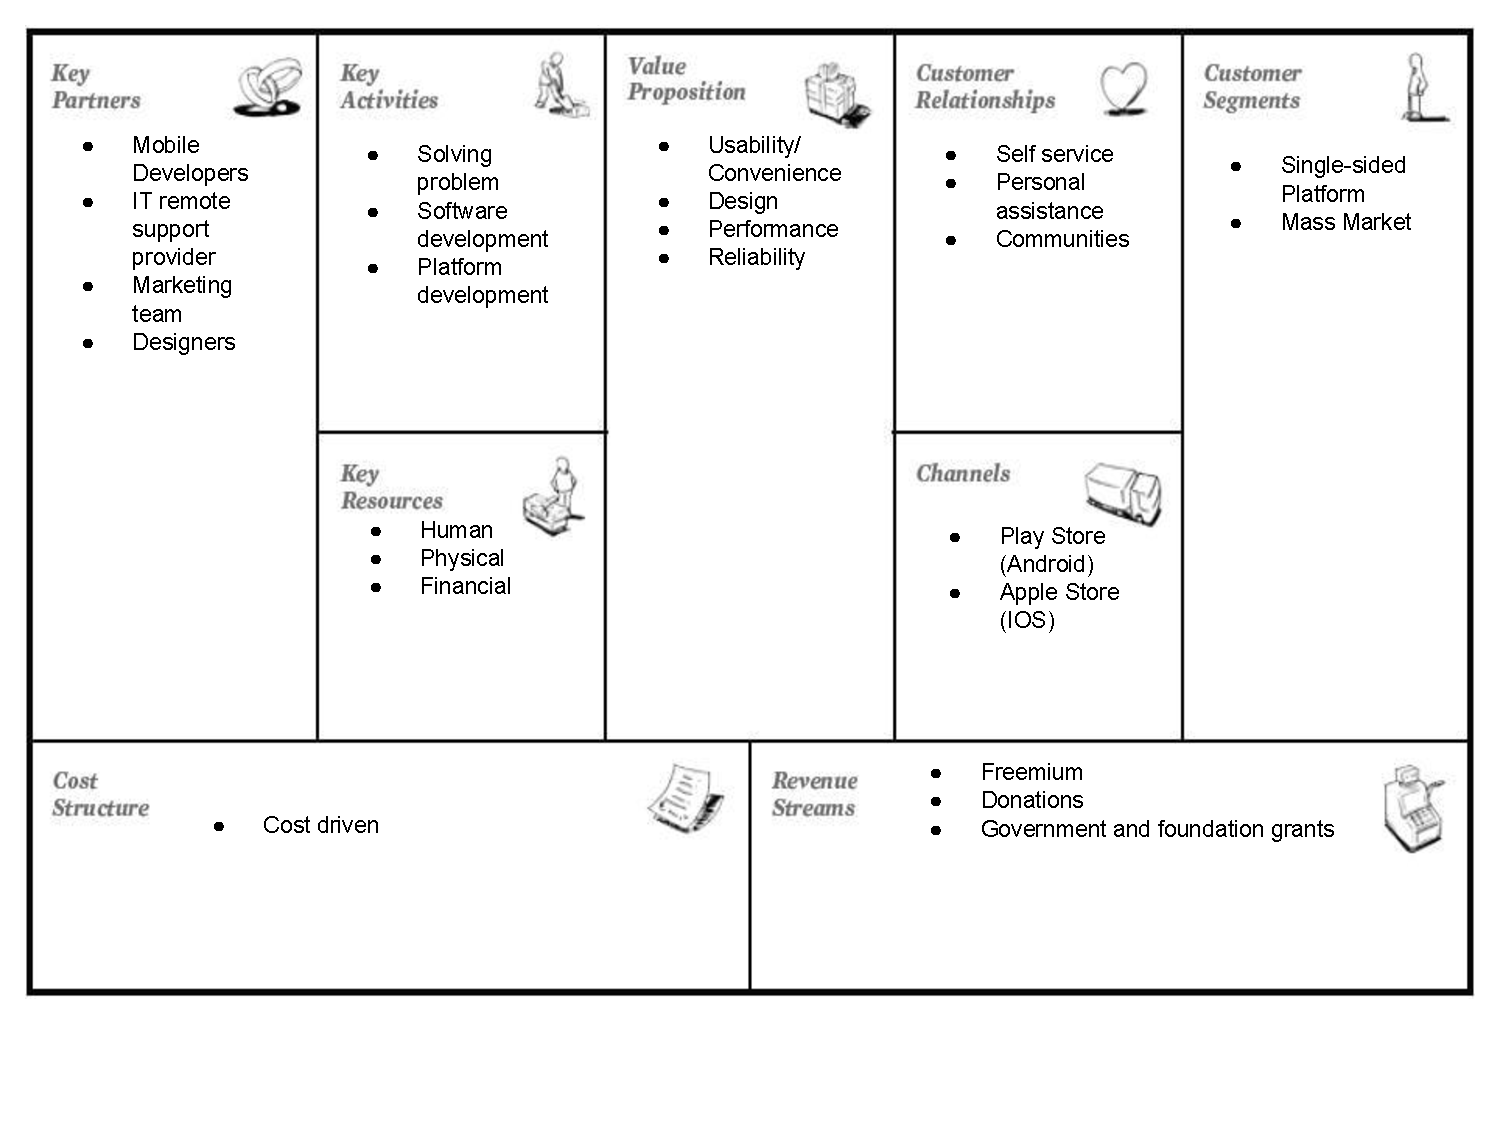
\includegraphics[height=.8\textheight]{img3/RBM.pdf}
}
\end{frame}

\section{Prototype}
\subsection{Actual Prototype}
\begin{frame}{Actual Prototype}{Relevium App Design}
  \begin{figure}[ht!]
    \begin{tcolorbox}[beamer,
                  width=0.8\textheight,
                  arc=2pt,
                  boxsep=0pt,
                  left=0pt,right=0pt,top=4pt,bottom=4pt,
                  ]
    \centering
    \includegraphics<1-3>[height=0.6\textheight]{AppDesign/actualDesign/AppMain.jpg}
    \only<1-3>{\quad}
    \includegraphics<2>[height=0.6\textheight]{AppDesign/actualDesign/Map.jpg}
    \includegraphics<3-4>[height=0.6\textheight]{AppDesign/actualDesign/AgentBlank.jpg}
    \only<4>{\quad}
    \includegraphics<4>[height=0.6\textheight]{AppDesign/actualDesign/AgentResponse.jpg}
    \only<1>{\caption{Relevium Home Screen}}
    \only<2>{\caption{Click ``\textbf{Map}"}}
    \only<3>{\caption{Click ``\textbf{Agent}"}}
    \only<4>{\caption{Live ``\textbf{Agent}"}}
    \label{fig:Actual_Draft}%
    \end{tcolorbox}
  \end{figure}
\end{frame}

\subsection{Expected Prototype}
\begin{frame}{Expected Prototype}
  \begin{figure}[ht!]
  \begin{tcolorbox}[beamer,
                  width=0.8\textheight,
                  arc=2pt,
                  boxsep=0pt,
                  left=0pt,right=0pt,top=4pt,bottom=4pt,
                  ]
    \centering
    \includegraphics<1->[height=0.6\textheight]{AppDesign/expectedDesign/1.png}
    \only<1->{\quad}
    \includegraphics<2>[height=0.6\textheight]{AppDesign/expectedDesign/2.png}
    \includegraphics<3>[height=0.6\textheight]{AppDesign/expectedDesign/3.png}
   \only<1>{\caption{Relevium Home Screen}}
    \only<2>{\caption{Chat ``\textbf{Agent}"}}
    \only<3>{\caption{Features List}}
    \label{fig:Expected_Draft}%
    \end{tcolorbox}
  \end{figure}
\end{frame}



\section{Live Demo}



\section{References}
\begin{frame}[shrink]{References}
\begin{itemize}

    \item https://github.com/MohamedEL-Torky/Prototype1 
    
    \item https://strategyzer.uservoice.com/how-do-i-use-the-key-partnerships-building-block-o
    \item https://hbr.org/2014/05/making-freemium-work
    \item https://grantspace.org/resources/knowledge-base/how-are-nonprofits-funded/
\end{itemize}
\end{frame}


\section*{Questions?}

\end{document}